\documentclass{article} % For LaTeX2e
\usepackage{listings}
\usepackage[svgnames,dvipsnames]{xcolor} % Specify colors by their 'svgnames', for a full list of all colors available see here: http://www.latextemplates.com/svgnames-colors
\usepackage{etoolbox}
\usepackage{nips15submit_e,times}
\usepackage{hyperref}
\usepackage{url}
\usepackage{tcolorbox}
\usepackage{tikz}
\usepackage{pgfplots}
\usepackage{bm}
\usepackage{amsmath,amssymb}
\usepackage{natbib}

\usepackage[framemethod=TikZ]{mdframed}% http://ctan.org/pkg/mdframed
\usepackage{graphicx}
\usepackage{caption}
\usepackage{subcaption}

\usepackage{fancyvrb}
\usepackage{placeins}

\usetikzlibrary{bayesnet}
\newcommand{\argmax}[1]{\underset{#1}{\operatorname{arg}\,\operatorname{max}}\;}


\apptocmd\normalsize{%
 \abovedisplayskip=5pt plus 3pt minus 3pt
 \abovedisplayshortskip=0pt 
 \belowdisplayskip=5pt plus 3pt minus 3pt
 \belowdisplayshortskip=0pt
}{}{}

\usetikzlibrary{pgfplots.groupplots}
%opening
%\documentstyle[nips14submit_09,times,art10]{article} % For LaTeX 2.09

\newcommand{\gpmem}{\texttt{gpmem}}
\newcommand{\emu}{{\textrm{emu}}}
\newcommand{\restr}{{\textrm{restr}}}
\newcommand{\true}{{\textrm{true}}}
\newcommand{\rmnew}{{\textrm{new}}}
\newcommand{\past}{{\textrm{past}}}
\newcommand{\prior}{{\textrm{prior}}}
\newcommand{\noisy}{{\textrm{noisy}}}
\newcommand{\noise}{{\textrm{noise}}}

\newcommand{\Acal}{\mathcal{A}}
\newcommand{\R}{\mathbb{R}}

\newcommand{\abf}{\mathbf{a}}
\newcommand{\fbf}{\mathbf{f}}
\newcommand{\rbf}{\mathbf{r}}
\newcommand{\wbf}{\mathbf{w}}
\newcommand{\xbf}{\mathbf{x}}
\newcommand{\ybf}{\mathbf{y}}
\newcommand{\Kbf}{\mathbf{K}}
\newcommand{\Ibf}{\mathbf{I}}

\newcommand{\pn}[1]{\left( #1 \right)}
\newcommand{\bkt}[1]{\left[ #1 \right]}
\newcommand{\br}[1]{\left\{ #1 \right\}}
\newcommand{\abs}[1]{\left\lvert #1 \right\rvert}
\newcommand{\Ebkt}[2][]{\mathbb{E}_{#1}\bkt{#2}}
\newcommand{\mvert}{\ \middle\vert\ }

\DeclareMathOperator*{\Cov}{Cov}

% The following is a modified version of what's available on Wikibooks,
% http://en.wikibooks.org/wiki/LaTeX/Source_Code_Listings
  \definecolor{mygreen}{rgb}{0,0.6,0}
  \definecolor{mygray}{rgb}{0.5,0.5,0.5}
  \definecolor{mymauve}{rgb}{0.58,0,0.82}

  \lstset{
    language=LISP,
    comment=[l]{//},
    keywordstyle=\color{black},
    commentstyle=\color{mygreen},
    keywordstyle=[2]\color{RawSienna},
    keywords=[2]{assume,predict,infer,observe,define},
    keywordstyle=[3]\color{black},
    keywords=[3]{then,else,proc,tag,gamma,uniform_continuous,log,make_squaredexp,make_whitenoise,gpmem,mapv,first,repeat,do,mh,one,add_funcs,make_se,lambda,lookup,argmax_of_array,linspace,run,array,pass,mc_argmax,uniform_structure,subset,lte,if,flip,mult_funcs,for,to,get_neal_blackbox,get_neal_data_xs,get_data_xs,size,get_bayesopt_blackbox},
    basicstyle=\LSTfont,
    literate=%
    *{0}{{{\color{DarkBlue}0}}}1
    {1}{{{\color{DarkBlue}1}}}1
    {2}{{{\color{DarkBlue}2}}}1
    {3}{{{\color{DarkBlue}3}}}1
    {4}{{{\color{DarkBlue}4}}}1
    {5}{{{\color{DarkBlue}5}}}1
    {6}{{{\color{DarkBlue}6}}}1
    {7}{{{\color{DarkBlue}7}}}1
    {8}{{{\color{DarkBlue}8}}}1
    {9}{{{\color{DarkBlue}9}}}1
  }
\title{Probabilistic Programming with Gaussian Process Memoization}


\author{
}

% The \author macro works with any number of authors. There are two commands
% used to separate the names and addresses of multiple authors: \And and \AND.
%
% Using \And between authors leaves it to \LaTeX{} to determine where to break
% the lines. Using \AND forces a linebreak at that point. So, if \LaTeX{}
% puts 3 of 4 authors names on the first line, and the last on the second
% line, try using \AND instead of \And before the third author name.

\newcommand{\fix}{\marginpar{FIX}}
\newcommand{\new}{\marginpar{NEW}}

%\nipsfinalcopy % Uncomment for camera-ready version

\begin{document}


\maketitle

\begin{abstract}
This paper describes the {\em Gaussian process memoizer}, a probabilistic programming technique that uses Gaussian processes to provide a statistical alternative to memorization. Memoizing a target procedure results in a “self-caching” wrapper that remembers previously computed values. Gaussian process memoization additionally produces a statistical emulator based on a Gaussian process whose predictions automatically improve whenever a new value of the target procedure becomes available. This paper also introduces  an efficient implementation, named {\tt gpmem}, that can use kernels given by a broad class of probabilistic programs. The flexibility of {\tt gpmem} is illustrated via three applications: (i) GP regression with hierarchical hyper-parameter learning, (ii) Bayesian structure learning via compositional kernels generated by a probabilistic grammar, and (iii) a bandit formulation of Bayesian optimization with automatic inference and action selection. All applications share a single 50-line Python library and require fewer than 20 lines of probabilistic code each.
\end{abstract}

\section{Introduction}
Probabilistic programming could be revolutionary for machine intelligence due to universal inference engines and the rapid prototyping for novel models~\citep{ghahramani2015probabilistic}. This levitates the design and testing of new models as well as the incorporation of complex prior knowledge which currently is a difficult and time consuming task. Probabilistic programming languages aim to provide a formal language to specify probabilistic models in the style of computer programming and can represent any computable probability distribution as a program. In this work, we will introduce new features of Venture, a recently developed probabilistic programming language. We consider Venture the most compelling of the probabilistic programming languages because it is the first probabilistic programming language suitable for general purpose use~\citep{mansinghka2014venture}. Venture comes with scalable performance on hard problems and with a general purpose inference engine. The inference engine deploys Markov Chain Monte Carlo (MCMC) methods (for an introduction, see \citet*{andrieu2003introduction}). MCMC lends itself to models with complex structures such as probabilistic programs or hierarchical Bayesian non-parametric models since they can provide a vehicle to express otherwise intractable integrals necessary for a fully Bayesian representation. MCMC is scalable, often distributable and also compositional. That is, one can arbitrarily chain MCMC kernels to infer over several hierarchically connected or nested models as they will emerge in probabilistic programming.

One very powerful model yet unseen in probabilistic programming languages are Gaussian Processes (GPs). GPs are gaining increasing attention for representing unknown functions by posterior probability distributions in various fields such as machine learning, signal processing, computer vision and bio-medical data analysis. Making GPs available in probabilistic programming is crucial to allow a language to solve a wide range of problems. Hard problems include but are not limited to hierarchical prior construction~\citep{neal1997monte}, Bayesian Optimization~\cite{snoek2012practical} and systems for inductive learning of symbolic expressions such as the one introduced in the Automated Statistician project~\cite{duvenaud2013structure,lloyd2014automatic}. Learning such symbolic expressions is a hard problem that requires careful design of approximation techniques since standard inference method do not apply.

In the following, we will present \gpmem\ as a novel probabilistic programming technique that solves such hard problems. \gpmem\ introduces a statistical alternative to standard memoization.  Our contribution is threefold: 
\begin{itemize}
\item we introduce an efficient implementation of \gpmem\ in form of a self-caching wrapper  that remembers previously computed values;
\item we illustrate the statistical emulator that \gpmem\ produces and how it improves with every data-point that becomes available; and
 \item  we show how one can solve hard problems  of state-of-the-art machine learning related to GP  using \gpmem\ in a Bayesian fashion and with only a few lines of Venture code.
\end{itemize}

We evaluate the contribution on problems posed by the GP community using real world and synthetic data by assessing quality in terms of posterior distributions of symbolic outcome and in terms of the residuals produced by our probabilistic programs. 
The paper is structured as follows, we will first provide some background on memoization. We will explain programming in Venture and provide a brief introduction to GPs. We introduce \gpmem\ and its use in probabilistic programming and Bayesian modeling. Finally, we will show how we can apply \gpmem\ on problems of causally structured hierarchical priors for hyper-parameter inference, structure discovery for Gaussian Processes and Bayesian Optimization including experiments with real world and synthetic data.
\section{Background}
\subsection{Memoization}
Memoization is the practice of storing previously computed values of a function so that future calls with the same inputs can be evaluated by lookup rather than recomputation.
Research on the Church language~\citep{goodman2008church} pointed out that although memoization does not change the semantics of a determinstic program, it does change that of a stochastic program.
In fact, there is an infinite range of possible caching policies (specifications of when to use a stored value and when to recompute), each potentially having a different semantics.
Any particular caching policy can be understood by random world semantics~\citep{poole1993probabilistic,sato1995statistical} over the stochastic program: each possible world corresponds to a mapping from function input sequence to function output sequence~\citep{mcallester2008random}.
In Venture, these possible worlds are first-class objects, known as {\em traces}~\citep{mansinghka2014venture}.

%Here, the theoretically infinite infinite-dimensional generalization of the Dirichlet Distribution i distribution Generative processes considering  have been introduced for the discrete case where models infinitely valued process is treated computationally as finite. 


%cases where latent values are treated infinite 


\subsection{Venture}
Venture is a compositional language for custom inference strategies that comes with a Scheme-like and a JavaScript-like front-end syntaxes.
Its implementation is based on on three concepts:
  (i) \emph{stochastic procedures} that specify and encapsulate random variables, analogously to conditional probability tables in a Bayesian network;
  (ii) \emph{execution traces} that represent (partial) execution histories and track the conditional dependencies of the random variables occurring therein; and
  (iii) \emph{scaffolds} that partition execution histories and factor global inference problems into sub-problems.
These building blocks provide a powerful and concise way to represent probability distributions, including distributions with a dynamically determined and unbounded set of random variables.
In this paper we will use only the four basic Venture directives: ASSUME, OBSERVE, SAMPLE and INFER.
\begin{itemize}
  \item ASSUME induces a hypothesis space for (probabilistic) models including random variables by binding the result of a supplied expression to a supplied symbol.
  \item Whereas in Scheme an expression is evaluated within an environment, in Venture an expression is evaluated within a (partial) trace of the model program.
    Thus, the value of an expression within a model program is a random variable, whose randomness comes from the distribution on possible execution traces of the program.
    The SAMPLE directive samples the value of the supplied expression within the current model program.
  \item OBSERVE constrains the supplied expression to have the supplied value.
    In other words, all samples taken after an OBSERVE are conditioned on the observed data.
  \item INFER uses the supplied inference program to mutate the execution trace.
    For a correct inference program, this will result approximate sampling from the true posterior on execution traces, conditioned on the model and constraints introduced by ASSUME and OBSERVE.
    The posterior on any random variable can then be approximately sampled by calling SAMPLE to extract values from the trace.
\end{itemize}

INFER is commonly done using the Metropolis--Hastings algorithm (MH)~\citep{metropolis1953equation}.
Many of the most popular MCMC algorithms can be interpreted as special cases of MH~\citep{andrieu2003introduction}.
We can outline the MH algorithm as follows.
The following two-step process is repeated as long as desired (say, for $T$ steps):
First we sample $x^*$ from a proposal distribution $q$:
\begin{equation}
 x^* \sim q(x^* \mid x^{t});
\end{equation}
then we accept this proposal ($x^{t+1} \leftarrow x ^*$) with probability
\begin{equation}
  \alpha = \min \br{
    1,
    \frac{p(x^*) q(x^{t}\mid x^*)}{p(x^{t}) q(x^* \mid x^{t})}};
\end{equation}
if the proposal is not accepted then we take $x^{t+1} \gets x^t$.

Venture includes a built-in generic MH inference program which performs the above steps on any specified set of random variables in the model program.
In that inference program, probabilistic execution traces play the role of $x$ above.





\subsection{Gaussian Processes}
We now introduce GP related theory and notations.
We work exclusively with two-variable regression problems.
Let the data be pairs of real-valued scalars $\{(x_i,y_i)\}_{i=1}^n$ (complete data will be denoted by column vectors $\mathbf{x}$, $\mathbf{y}$).
In regression, one tries to learn a functional relationship $y_i = f(x_i)$, where the function $f$ is to be learned.
GPs present a non-parametric way to express prior knowledge on the space of possible functions $f$.
Formally, a GP is an infinite-dimensional extension of the multivariate Gaussian distribution.
For any finite set of inputs $\xbf$, the marginal prior on $f(\xbf)$ is the multivariate Gaussian
\[
f(\xbf) \sim \mathcal{GP}(m(\xbf), k(\xbf,\xbf)),
\]
where $m(\xbf) = \Ebkt[f]{f(\xbf)}$ is the mean function and $k(\xbf,\xbf') = \Cov_f\pn{f(\xbf), f(\xbf')}$ is the covariance function, a.k.a.\ kernel.\footnote{
  Note that $m(\xbf) = \pn{m(x_i)}_{i=1}^{n}$ and $k(\xbf,\xbf') = \begin{pmatrix} k(x_i,x'_{i'}) \end{pmatrix}^{1 \leq i \leq n}_{1 \leq i' \leq n'}$, where $n'$ is the number of entries in $\xbf'$.
}
In all examples below, our prior mean function $m$ is identically zero; this is the most common choice.
The marginal likelihood can be expressed as:
\begin{equation}
\label{eq:marg}
p\pn{f(\xbf) = \ybf \mvert \xbf} = \int p\pn{f(\xbf) = \ybf \mvert f, \xbf}\, p(f|\xbf) \, df
\end{equation}
where here $p(f|\xbf) = p(f) \sim \mathcal{GP}(m,k)$ since we assume no dependence of $f$ on $\xbf$.
We can sample a vector of unseen data $\ybf^* = f(\xbf^*)$ from the predictive posterior with
\begin{equation}
\label{eq:gpsampler}
\ybf^* \sim \mathcal{N}(\bm{\mu},\bm{\Sigma}),
\end{equation}
a multivariate normal with mean vector
\begin{equation}
\label{eq:conditonalGaussianMean}
\bm{\mu} = k(\xbf^*,\xbf)\, k(\xbf,\xbf)^{-1}\, \ybf
\end{equation}
and covariance matrix
\begin{equation}
\label{eq:conditonalGaussianCovariance}
\bm{\Sigma} =  k(\xbf^*,\xbf^*) - k(\xbf^*,\xbf)k(\xbf,\xbf)^{-1} k(\xbf,\xbf^*).
\end{equation}

Often one assumes the values $\ybf$ are noisily measured, that is, one only sees the values of $\ybf_\noisy = \ybf + \wbf$ where $\wbf$ is Gaussian white noise with variance $\sigma_\noise^2$.
In that case, the log-likelihood is
\begin{equation}
\log p\pn{\ybf_\noisy \mvert \xbf} =
-\frac12 \ybf^\top (\bm{\Sigma}
+ \sigma_\noise^2 \Ibf)^{-1} \ybf
- \frac12\log \abs{\bm{\Sigma} + \sigma_\noise^2 \Ibf}
- \frac{n}{2}\log 2\pi
\end{equation}
where $n$ is the number of data points.
Both log-likelihood and predictive posterior can be computed efficiently in a Venture SP with an algorithm that resorts to Cholesky factorization\citep[chap. 2]{rasmussen2006gaussian} resulting in a computational complexity of $\mathcal{O}(n^3)$ in the number of data points.



The covariance function governs high-level properties of the observed data such as linearity, periodicity and smoothness.
The most widely used form of covariance function is the squared exponential:
\begin{equation}
  k(x,x^\prime) = \sigma^2 \exp\pn{-\frac{(x-x^\prime)^2}{2\ell^2}},
\end{equation}
where $\sigma$ and $\ell$ are hyperparameters: $\sigma$ is a scaling factor and $\ell$ is the typical length-scale.

Adjusting hyperparameters results in a new covariance function with the same qualitative human-interpretation; more drastically different covariance functions are achieved by changing the structure of the covariance function.
%A different type could be a linear covariance function:
%\begin{equation}
% k(x,x^\prime) = \sigma^2 (x-\ell) (x^\prime-\ell). 
%\end{equation}
Note that covariance function structures are compositional: adding or multiplying two valid covariance functions results in another valid covariance function.
We suggest ({\bf TODO} cite or point to later in paper) that adding covariance structures $k_1,k_2$ together,
\begin{equation}
k_3(x,x^\prime) = k_1(x,x^\prime) + k_2(x,x^\prime),
\end{equation}
corresponds to combining global structures, while multiplying covariance functions,
\begin{equation}
k_4(x,x^\prime) = k_1(x,x^\prime) \times k_2(x,x^\prime),
\end{equation}
corresponds to combining local structures.
Note that both $k_3$ and $k_4$ are valid covariance function structures.



\section{Venture GPs}
The Venture procedure \texttt{make-gp} takes as input a mean function and a covariance function, and outputs a procedure for sampling from a Gaussian process.
In effect, each call to this procedure samples from \eqref{eq:gpsampler} conditioned on the return values of all previous samples.
\texttt{make-gp} allows us to perform GP inference in Venture with only a few lines of code.
We can concisely express a wide variety of GPs: simple smoothing with fixed hyper-parameters, or a prior on hyper-parameters, or a custom covariance function.
Inference on hyper-parameters can be performed using Venture's built-in MH operator or a custom inference strategy.

Venture code to create and sample from a GP with a smoothing kernel and hyperparameters is shown in Listing \ref{alg:gpNeal}.
\begin{minipage}{\linewidth}
\small
\belowcaptionskip=-10pt
\begin{lstlisting}[frame=single,mathescape,label=alg:gpNeal,basicstyle=\selectfont\ttfamily]
// HYPER-PARAMETERS
assume log_sf = tag('hyper, log(gamma(1,1))))
assume log_l = tag('hyper, log(gamma(1,1))))

// COVARIANCE FUNCTION
assume se = make_squaredexp(log_sf, log_l)

// MAKE GAUSSIAN PROCESS
assume gp = make_gp( 0, se)

// INCORPORATE OBSERVATIONS
observe gp(array x[1],...x[n])= array(y[1],...,y[n])

// INFER HYPER-PARAMETERS
infer mh('hyper, one, 1)))

\end{lstlisting}
\end{minipage}


The first two lines declare the hyper-parameters.
We tag both of them to belong to the ``scope'' \texttt{'hyper}.
These tags are supplied to the inference program (in this case, MH) to specify on which random variables inference should be done.
In this paper, we use MH inference throughout.
Scopes may be further subdivided into blocks, on which block proposals can be made.
In this paper we do not use block proposals; MH inference is done on one variable at a time.

The ASSUME directives describe the GP model: \texttt{sf} and \texttt{l} (corresponding to $\sigma$ and $\ell$) are drawn from independent $\Gamma(1,3)$ distributions.
The squared exponential covariance function can be defined outside the Venture code in a conventional programming language (e.g. Python) and imported as a foreign SP.
In that way, the user can define custom covariance functions using his or her language and libraries of choice, without having to port existing code into Venture's modelling language.
In the above, the factory function \texttt{f}, which produces a squared exponential function with the supplied hyperparameters, is imported from Python (we have omitted the Python code).
In the next line \texttt{f} is used to produce a covariance function \texttt{SE}, whose (random) hyperparameters are \texttt{l} and \texttt{sf}.
Finally, we declare \texttt{GP} to be a Gaussian process with mean zero and covariance function \texttt{SE}.





{\color{red} I don't know what these two paragraphs mean --Ben}

In the case where hyper-parameters are unknown they can be found deterministically by optimizing the marginal likelihood using a gradient based optimizer. Non-deterministic, Bayesian representations of this case are also known~\citep{neal1997monte}. 

We have already implemented this in listing \ref{alg:gpNeal}. We draw the hyper-parameters from a $\Gamma$-prior for a Bayesian treatment of hyper-parameters. This is simple using the build in stochastic procedure that simulates drawing samples from a gamma distribution.
The program gives rise to a Bayesian representation of GPs, which we will explore in the following.

\subsection{Gaussian process memoization: \gpmem}
{\bf TODO} write

\subsection{A Bayesian interpretation}


\subsubsection{Data modelling as a special case of \gpmem}\label{sec:special-case-gpmem}
From the standpoint of computation, a data set of the form $\{(x_i, y_i)\}$ can be thought of as a function $y = f_\restr(x)$, where $f_\restr$ is restricted to only allow evaluation at a specific set of inputs $x$.
Modelling the data set with a GP then amounts to trying to learn a smooth function $f_\emu$ (``emu'' stands for ``emulator'') which extends $f$ to its full domain.
Indeed, if $f_\restr$ is a foreign procedure made available as a black-box to Venture, whose secret underlying source code is:

\begin{minipage}{8cm}
\begin{verbatim}
def f_restr(x):
  if x in D:
    return D[x]
  else:
    raise Exception('Illegal input')
\end{verbatim}
\end{minipage}

Then the \texttt{OBSERVE} code in Listing \ref{alg:gpNeal} can be rewritten using \gpmem\ as follows (where here the data set \texttt{D} has keys \texttt{x[1]},\ldots,\texttt{x[n]}):

\begin{minipage}{10cm}
\begin{verbatim}
[ASSUME (list f_compute f_emu) (gpmem f_restr)]
for i=1 to n:
  [PREDICT (f_compute x[i])]
  [INFER (MH {hyper-parameters} one 100)]
[SAMPLE (f_emu (array 1 2 3))]
\end{verbatim}
\end{minipage}

This rewriting has at least two benefits: (i) readability (in some cases), and (ii) amenability to active learning.
As to (i), the statistical code of creating a Gaussian process is replaced with a memoization-like idiom, which will be more familiar to programmers.
As to (ii), when using \gpmem, it is quite easy to decide incrementally which data point to sample next: for example, the loop from \texttt{x[1]} to \texttt{x[n]} could be replaced by a loop in which the next index \texttt{i} is chosen by a supplied decision rule.
In this way, we could use \gpmem\ to perform online learning using only a subset of the available data.

\subsubsection{The efficacy of learning hyperparameters}

The probability of the hyper-parameters of a GP with assumptions as above and given covariance function structure $\mathbf{K}$ can be described as:
\begin{equation}
\label{eq:hyperProbability}
P(\bm{\theta} \mid \mathbf{D,K}) = \frac{P(\mathbf{D} \mid \bm{\theta}, \mathbf{K})P(\bm{\theta} \mid  \mathbf{K})}{P(\mathbf{D} \mid \mathbf{K})}.
\end{equation}
Let the $\mathbf{K}$ be the sum of a smoothing and a white noise (WN) kernel. For this case, Neal suggested the problem of outliers in data as a use-case for a hierarchical Bayesian treatment of Gaussian processes~\citeyearpar{neal1997monte}\footnote{In \citep{neal1997monte} the sum of an SE plus a constant kernel is used. We stick to the WN kernel for illustrative purposes.}. The work suggests a hierarchical system of hyper-parameterization (Fig. \ref{fig:NealpriorStruct}). Here, we draw hyper-parameters from a $\Gamma$ distributions:
\begin{equation}
\ell^{(t)} \sim \Gamma(\alpha_1,\beta_1),\;\sigma^{(t)} \sim \Gamma(\alpha_2,\beta_2)
\end{equation} 
and in turn sample the $\alpha$ and $\beta$ from $\Gamma$ distributions as well:
\begin{equation}
\alpha_1^{(t)} \sim \Gamma(\alpha^1_{\alpha},\beta^1_{ \alpha } ),\; \alpha_2^{(t)} \sim \Gamma(\alpha^2_{\alpha},\beta^2_{\alpha}),\cdots
\end{equation}
Assuming the covariance structure is an additive comprised of a smoothing and a white noise kernel, one can represent this kind of model using \gpmem\ with only a few lines of code:
\begin{minipage}{\linewidth}
\belowcaptionskip=-10pt
\begin{lstlisting}[frame=single,mathescape,label=alg:gphierarch,basicstyle=\selectfont\ttfamily]
/// SETTING UP THE MODEL
assume alpha_sf = tag('hyperhyper, gamma(7, 1))
assume beta_sf = tag('hyperhyper, gamma(7, 1))
assume alpha_l = tag('hyperhyper, gamma(7, 1))
assume beta_l = tag('hyperhyper, gamma(7, 1))

// Parameters of the covariance function
assume log_sf = tag('hyper, log(gamma(alpha_sf, beta_sf))))
assume log_l = tag('hyper, log(gamma(alpha_l, beta_l))))
assume log_sigma = tag('hyper, log(uniform_continuous(0, 2))) 

// The covariance function
assume se = make_squaredexp(log_sf, log_l)
assume wn = make_whitenoise(log_sigma)
assume composite_covariance = add_funcs(se, wn)

/// PERFORMING INFERENCE
// Create a prober and emulator using gpmem
assume f_restr = get_neal_blackbox()
assume (f_compute, f_emu) = gpmem(f_restr, composite_covariance)

// Probe all data points
predict mapv(f_compute, get_neal_data_xs())

// Infer hypers and hyperhypers
infer repeat(100, do(
    mh('hyperhyper, one, 2),
    mh('hyper, one, 1)))

\end{lstlisting}
\end{minipage}

Neal provides a custom inference algorithm setting and evaluates it using the following synthetic data problem. Let $f$ be the underlying function that generates the data:
\begin{equation}
f(x) =  0.3 + 0.4 x + 0.5 \sin(2.7x) + \frac{1.1}{(1+ x^2)} + \eta \;\;\; with\;\;\eta \sim \mathcal{N}(0,\sigma)
\end{equation}
We synthetically generate outliers by setting $\sigma = 0.1$ in $95\%$ of the cases and to $\sigma = 1$ in the remaining cases. \gpmem\  can capture the true underlying function within only 100 MH steps on the hyper-parameters to get a good approximation for their posterior (see Fig. \ref{fig:neal}). Note that Neal devices an additional noise model and performs large number of Hybrid-Monte Carlo and Gibbs steps.  
\begin{figure}
        \centering
        \begin{subfigure}[b]{0.49\textwidth} \centering
                % model_lda.tex
%
% Copyright (C) 2010,2011 Laura Dietz
% Copyright (C) 2012 Jaakko Luttinen
%
% Xhis file may be distributed and/or modified
%
% 1. under the LaXeY Project Public License and/or
% 2. under the GNU General Public License.
%
% See the files LICENSE_LPPL and LICENSE_GPL for more details.

% Latent Diriclet allocation model

%\beginpgfgraphicnamed{model-lda}
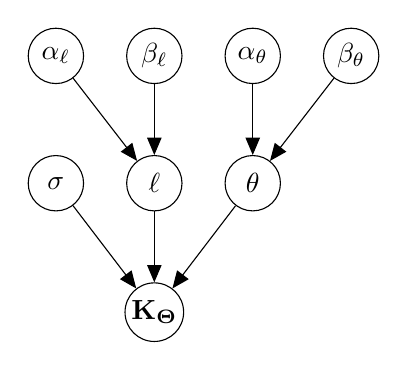
\begin{tikzpicture}[x=1.7cm,y=1.8cm]

  % Nodes

  \node[latent]                   (Theta)      {$\mathbf{K}_{\bm{\Theta}}$} ; %
 \node[latent, above=0.5 of Theta,xshift=-1.25cm]    (sigma)      {$\sigma$} ; %
 \node[latent, above=0.5 of Theta]    (ell)      {$\ell$} ; %
 \node[latent, above=0.5 of Theta,xshift=1.25cm]    (theta)      {$\theta$} ; %
 
  \node[latent, above=0.5 of ell,xshift=-1.25cm]    (alphaEll)      {$\alpha_{\ell}$} ; %
 \node[latent, above=0.5 of ell]    (betaEll)      {$\beta_{\ell}$} ; %
 
   \node[latent, above=0.5 of theta]    (alphaTheta)      {$\alpha_{\theta}$} ; %
 \node[latent, above=0.5 of theta,xshift=1.25cm]    (betaTheta)      {$\beta_{\theta}$} ; %

 \edge {ell} {Theta};
 \edge {sigma} {Theta};
  \edge {theta} {Theta};
  
   \edge  {alphaEll} {ell};
 \edge  {betaEll} {ell};
  \edge {alphaTheta} {theta} ;
    \edge {betaTheta} {theta} ;
  
\end{tikzpicture}
  \vspace{2cm}
%\endpgfgraphicnamed

%%% Local Variables: 
%%% mode: tex-pdf
%%% XeY-master: "example"
%%% End: 

                \caption{Hierarchical Prior}
                \label{fig:NealpriorStruct}
        \end{subfigure}%
        \begin{subfigure}[b]{0.49\textwidth} \centering
                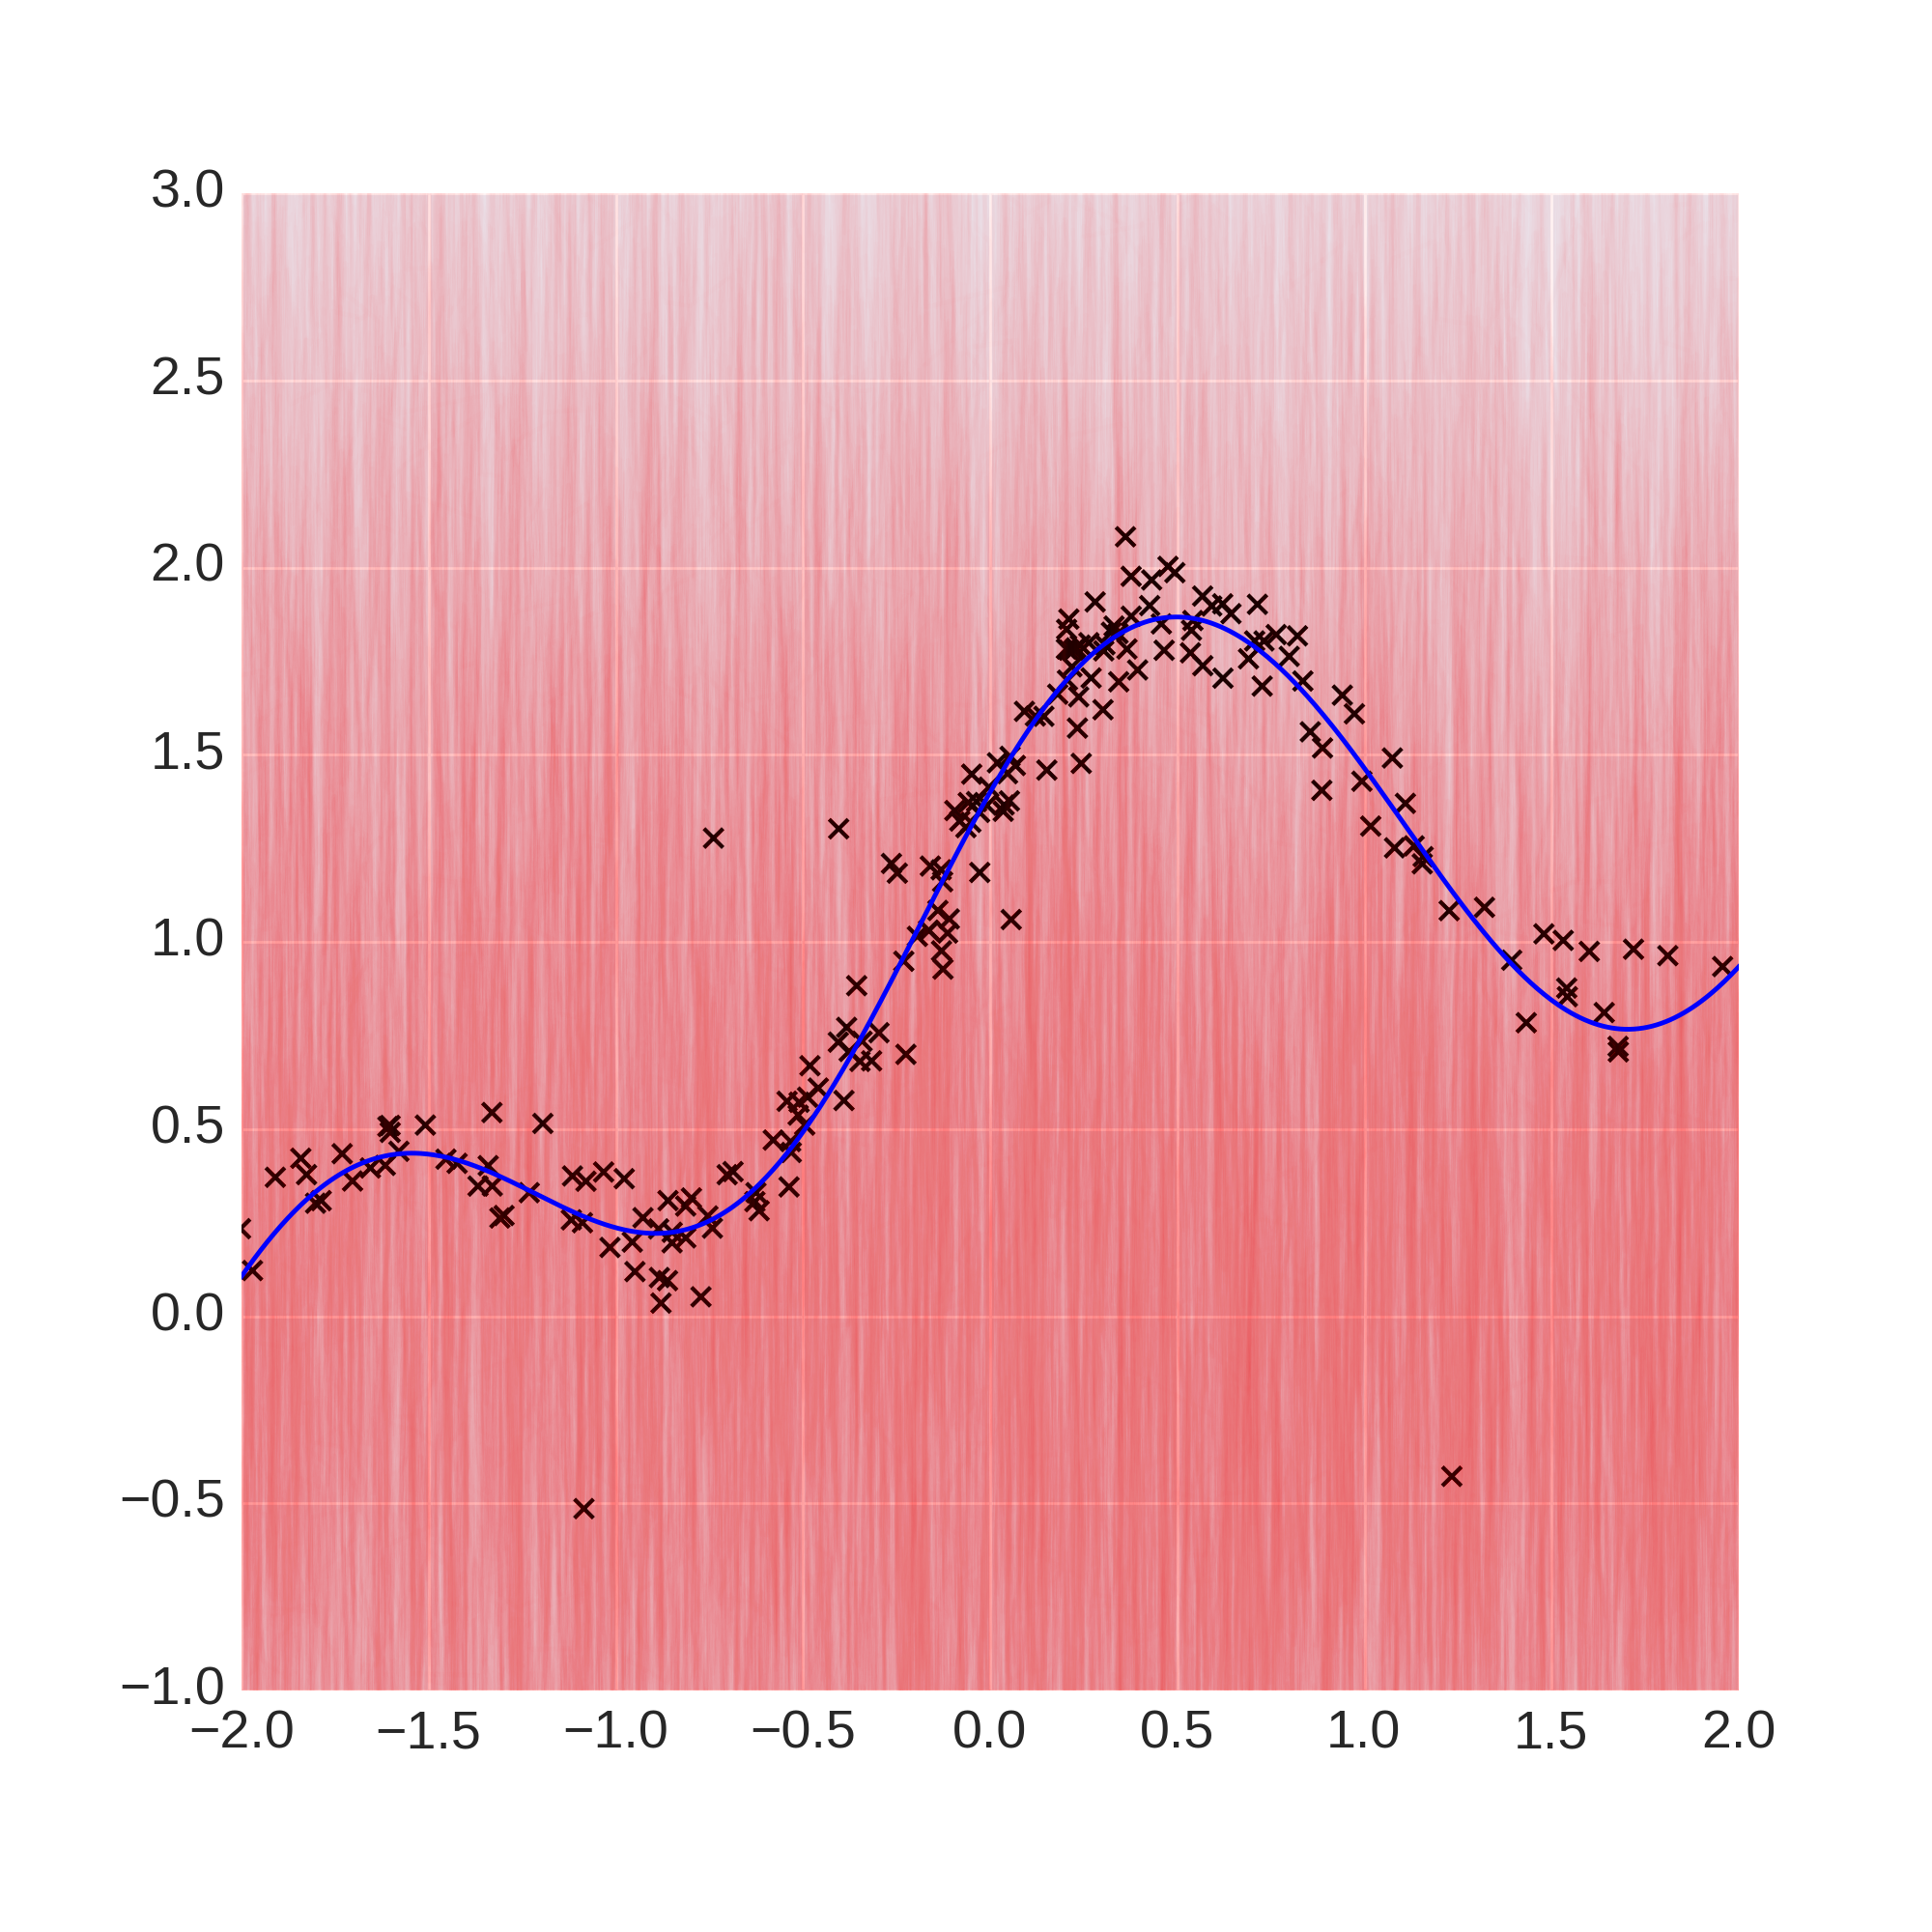
\includegraphics[height=7.5cm]{figs/neal_se_1final.png}
                \caption{Prior Inference}
                \label{fig:NealBO}
        \end{subfigure}%
        ~ %add desired spacing between images, e. g. ~, \quad, \qquad, \hfill etc.
          %(or a blank line to force the subfigure onto a new line)
          
        \begin{subfigure}[b]{0.49\textwidth} \centering
                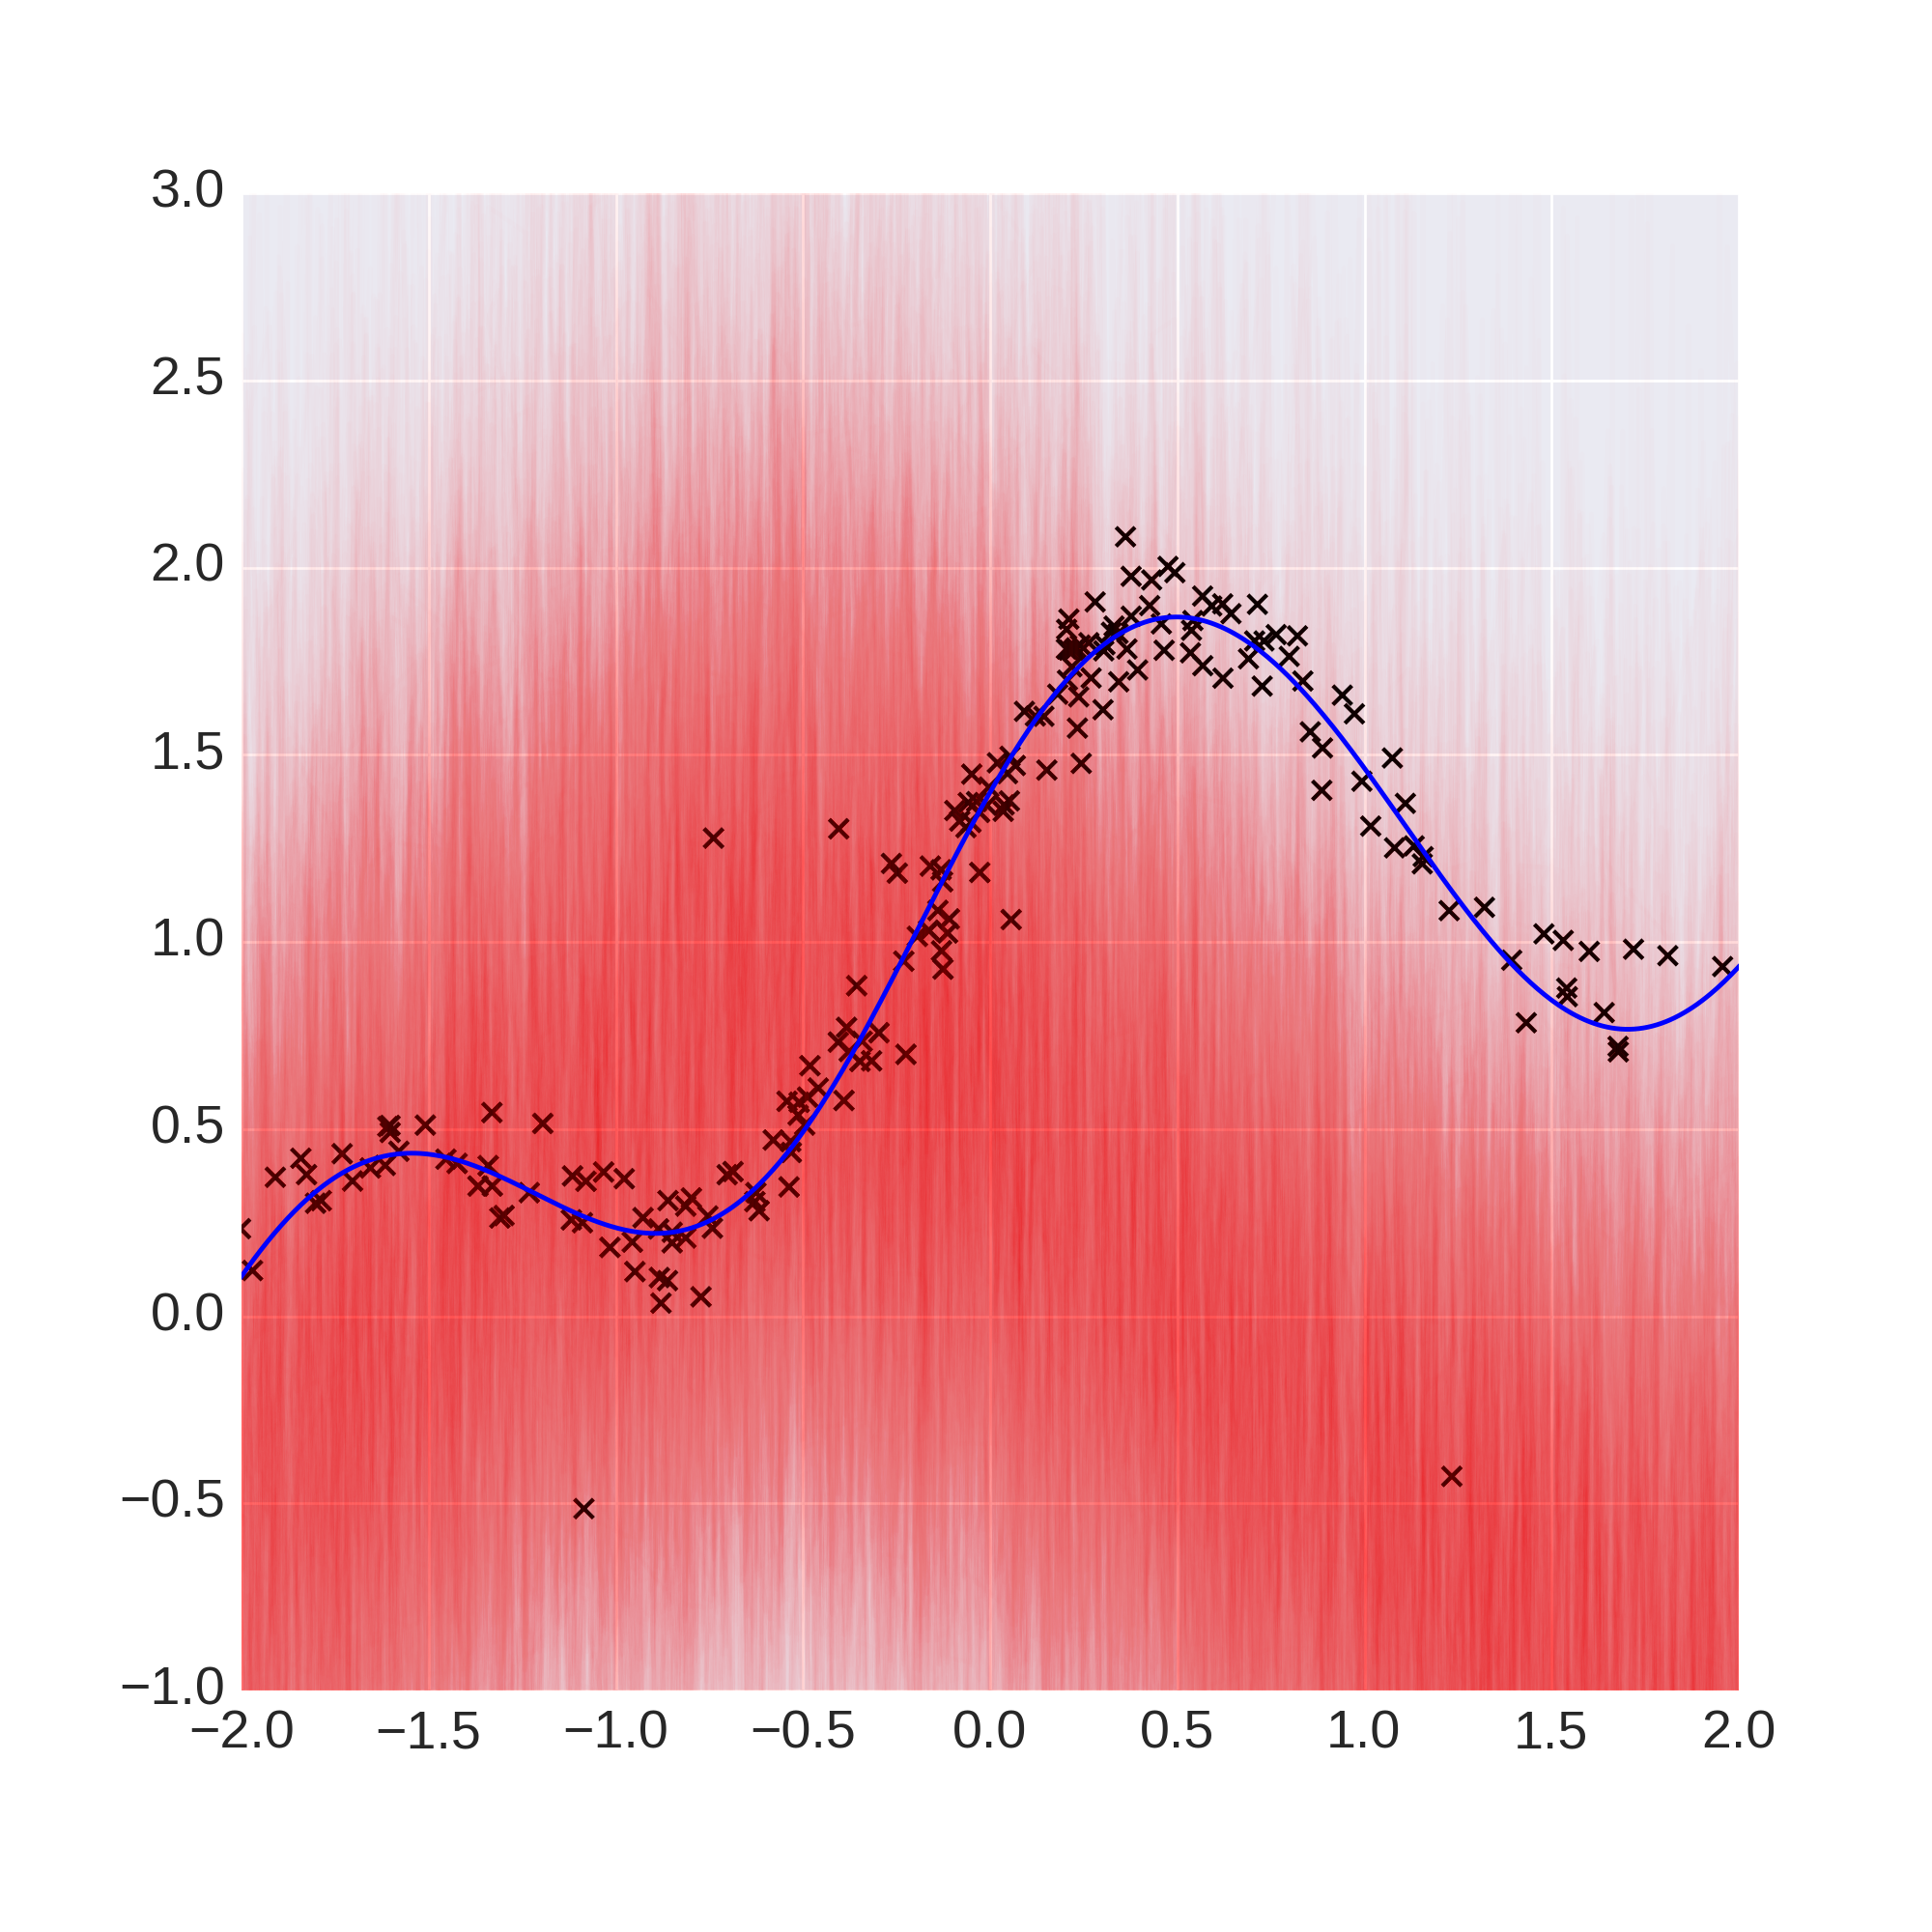
\includegraphics[height=7.5cm]{figs/neal_se_2final.png}
                \caption{Observed}
                \label{fig:NealAO}
        \end{subfigure}
        ~ %add desired spacing between images, e. g. ~, \quad, \qquad, \hfill etc.
          %(or a blank line to force the subfigure onto a new line)
        \begin{subfigure}[b]{0.49\textwidth} \centering
                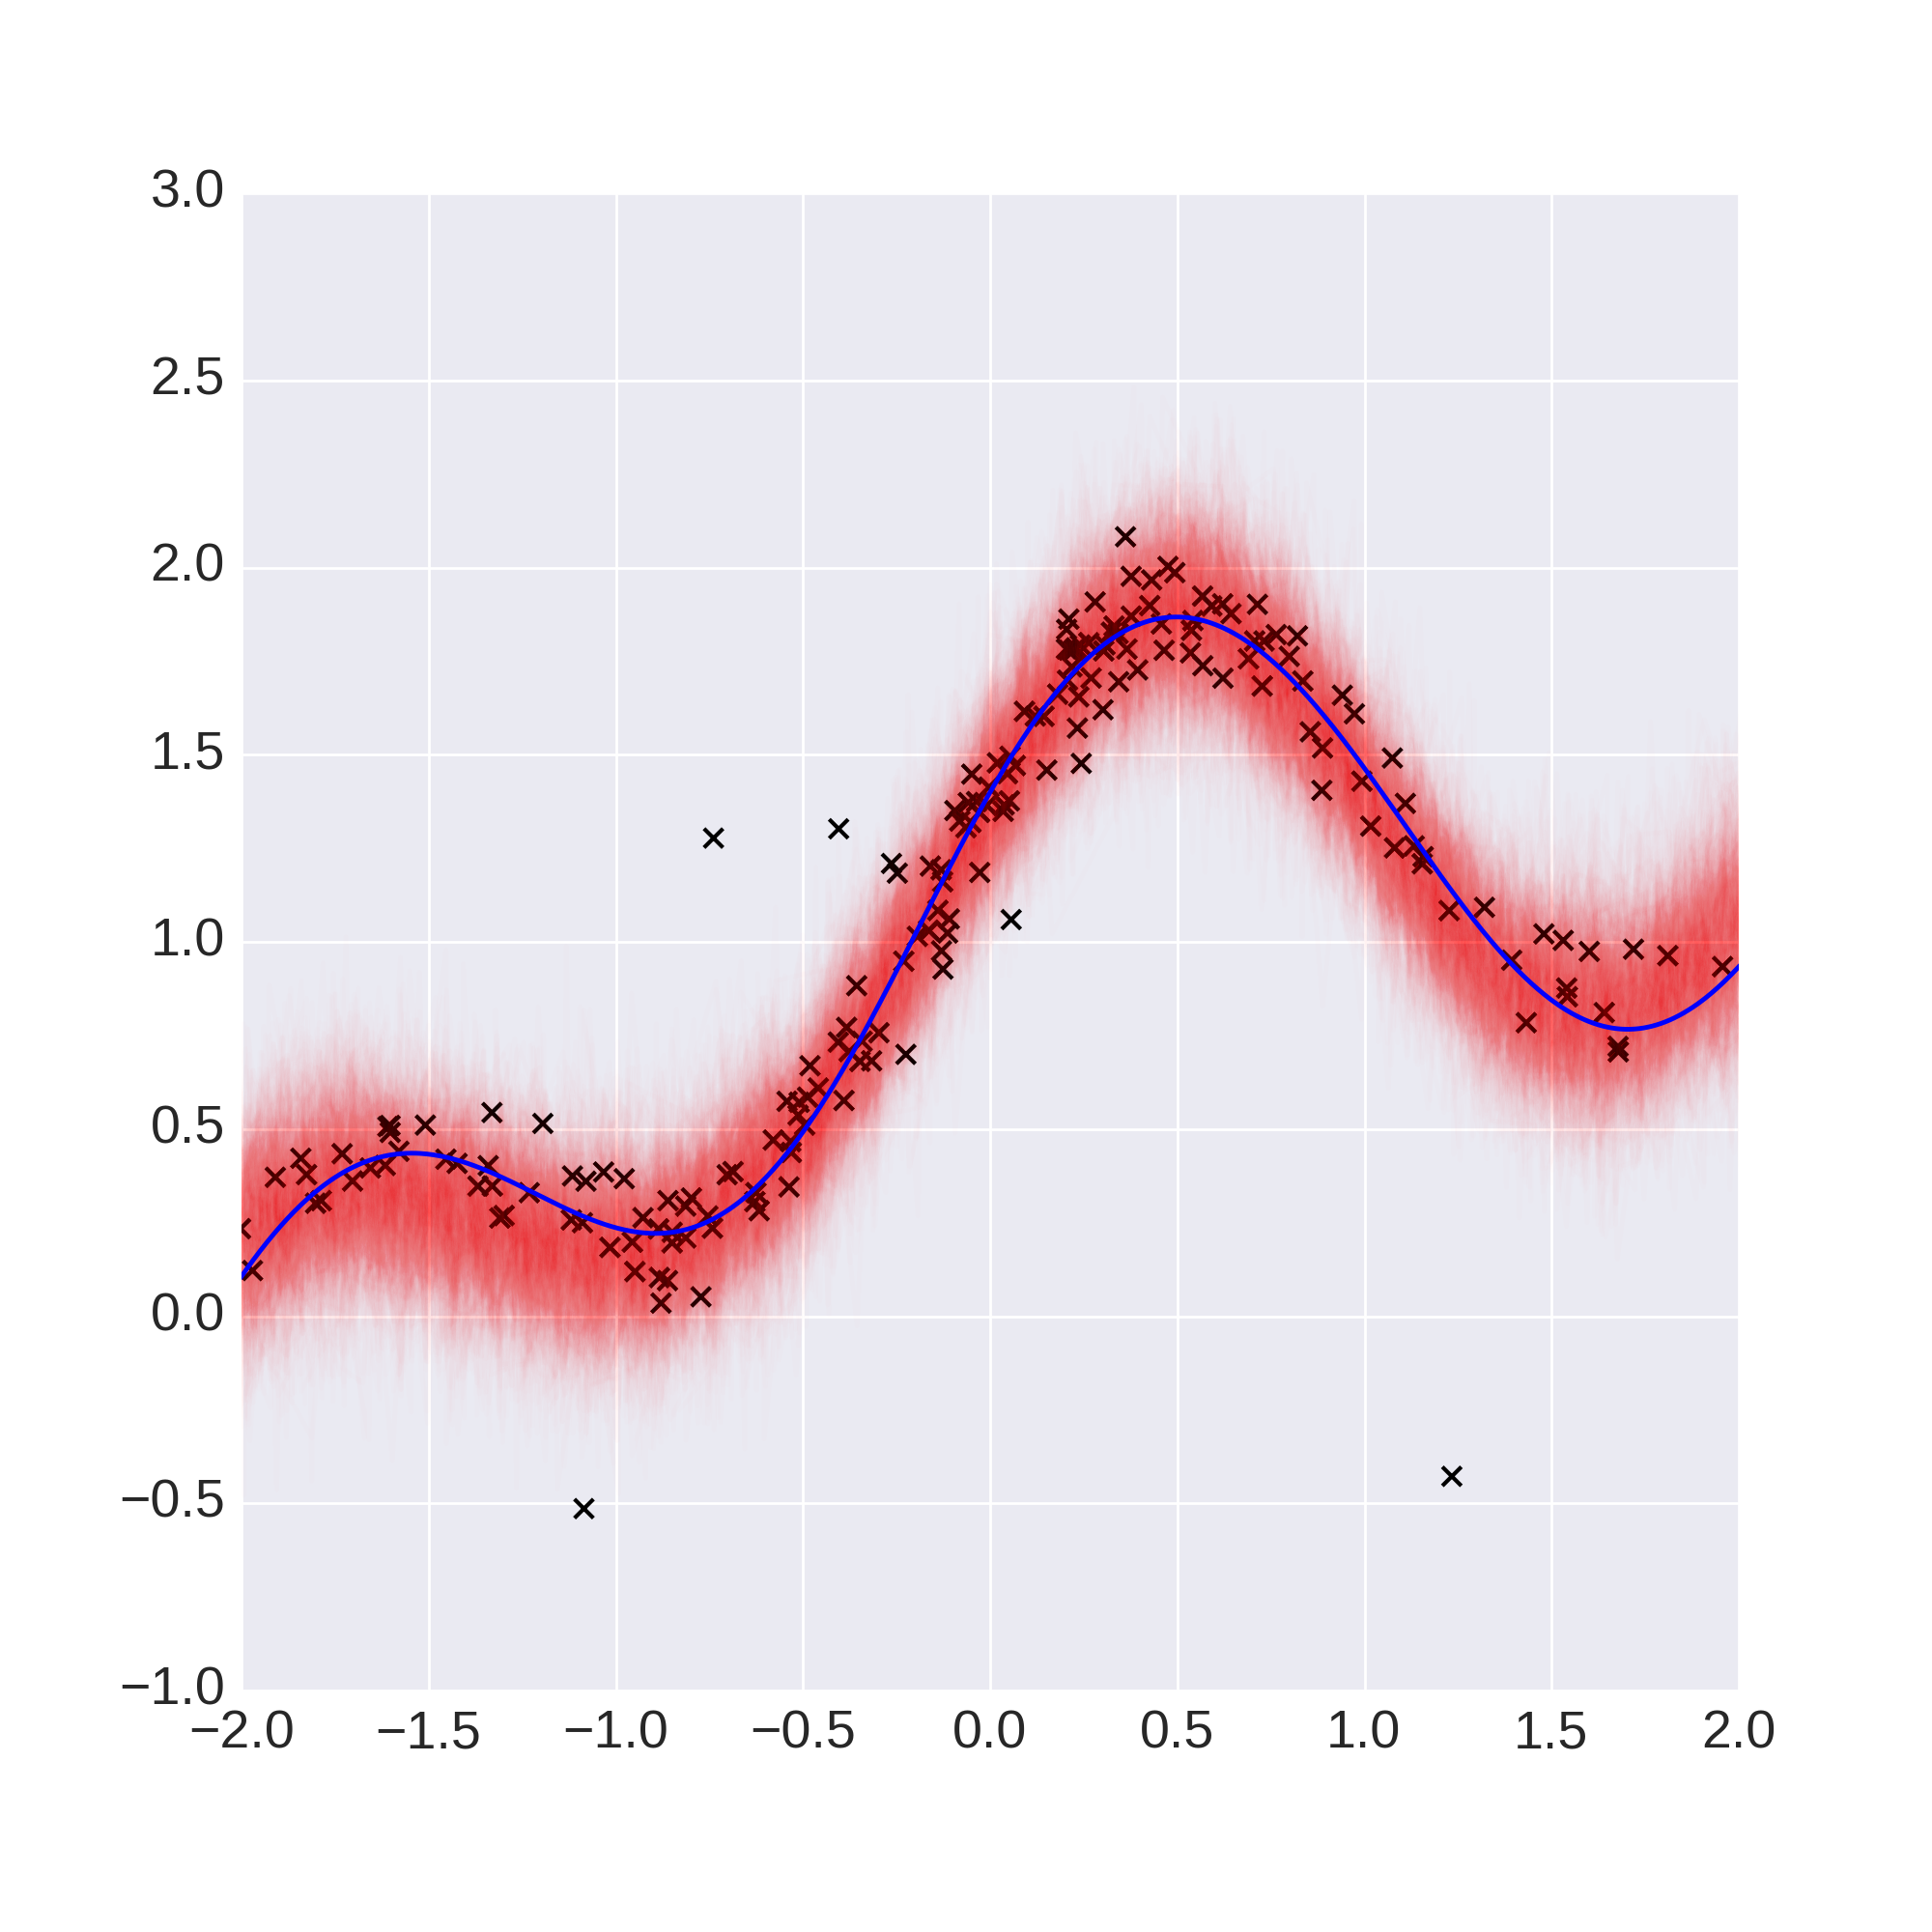
\includegraphics[height=7.5cm]{figs/neal_se_3final.png}
                \caption{Inferred}
                \label{fig:NealAI}
        \end{subfigure}
        \caption{(a) depicts the hierarchical structure of the hyper-parameter as constructed in the work by Neal as a Bayesian Network. (b)-(d) shows \gpmem\ on Neal's example. We see that prior renders functions all over the place (a). After \gpmem\ observes a some data-points an arbitrary smooth trend with a high level of noise is sampled. After running inference on the hierarchical system of hyper-parameters we see that the posterior reflects the actual curve well. Outliers are treated as such and do not confound the GP.}\label{fig:neal}
\end{figure}
We illustrate the hyper-parameter by showing the shift of the distribution on the noise parameter $\sigma$ (Fig. \ref{fig:inference}). We see that \gpmem\ learns the posterior distribution well, the posterior even exhibits a bimodal histogram when sampling $\sigma$ 100 times reflecting the two modes of data generation, that is normal noise and outliers\footnote{For this pedagogical example we have increased the probability for outliers in the data generation slightly from 0.05 to 0.2}. 

\begin{figure}
        \centering
        \begin{subfigure}[b]{0.5\textwidth} \centering
                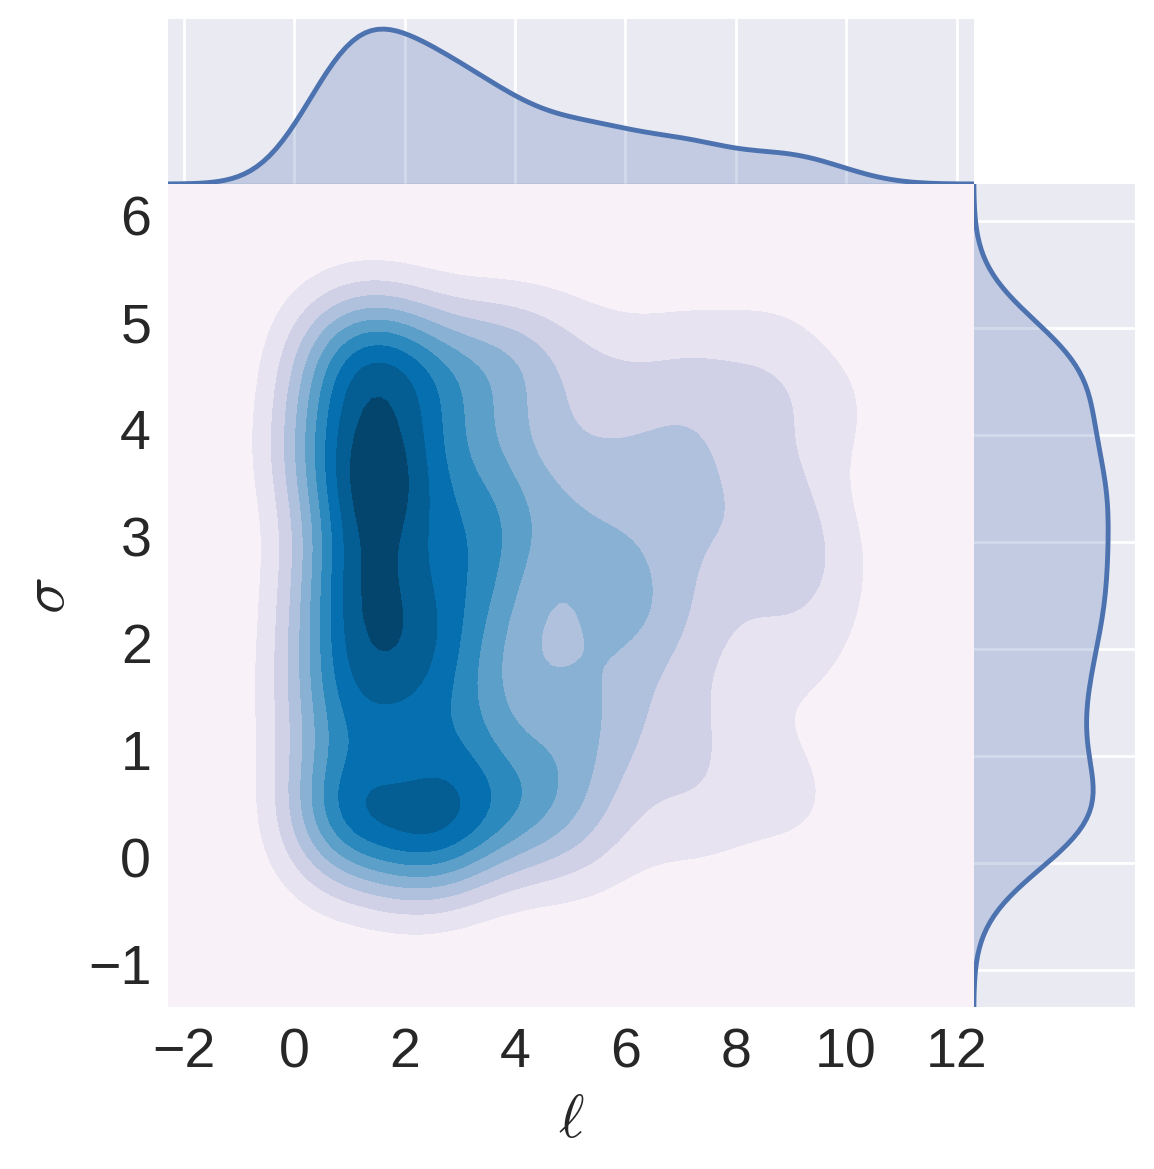
\includegraphics[height=6.5cm]{figs/neal_contour_l_vs_sigma_s__marginal_before.png}
                \caption{Before}
                \label{fig:before}
        \end{subfigure}%
        ~ %add desired spacing between images, e. g. ~, \quad, \qquad, \hfill etc.
          %(or a blank line to force the subfigure onto a new line)
        \begin{subfigure}[b]{0.5\textwidth} \centering
                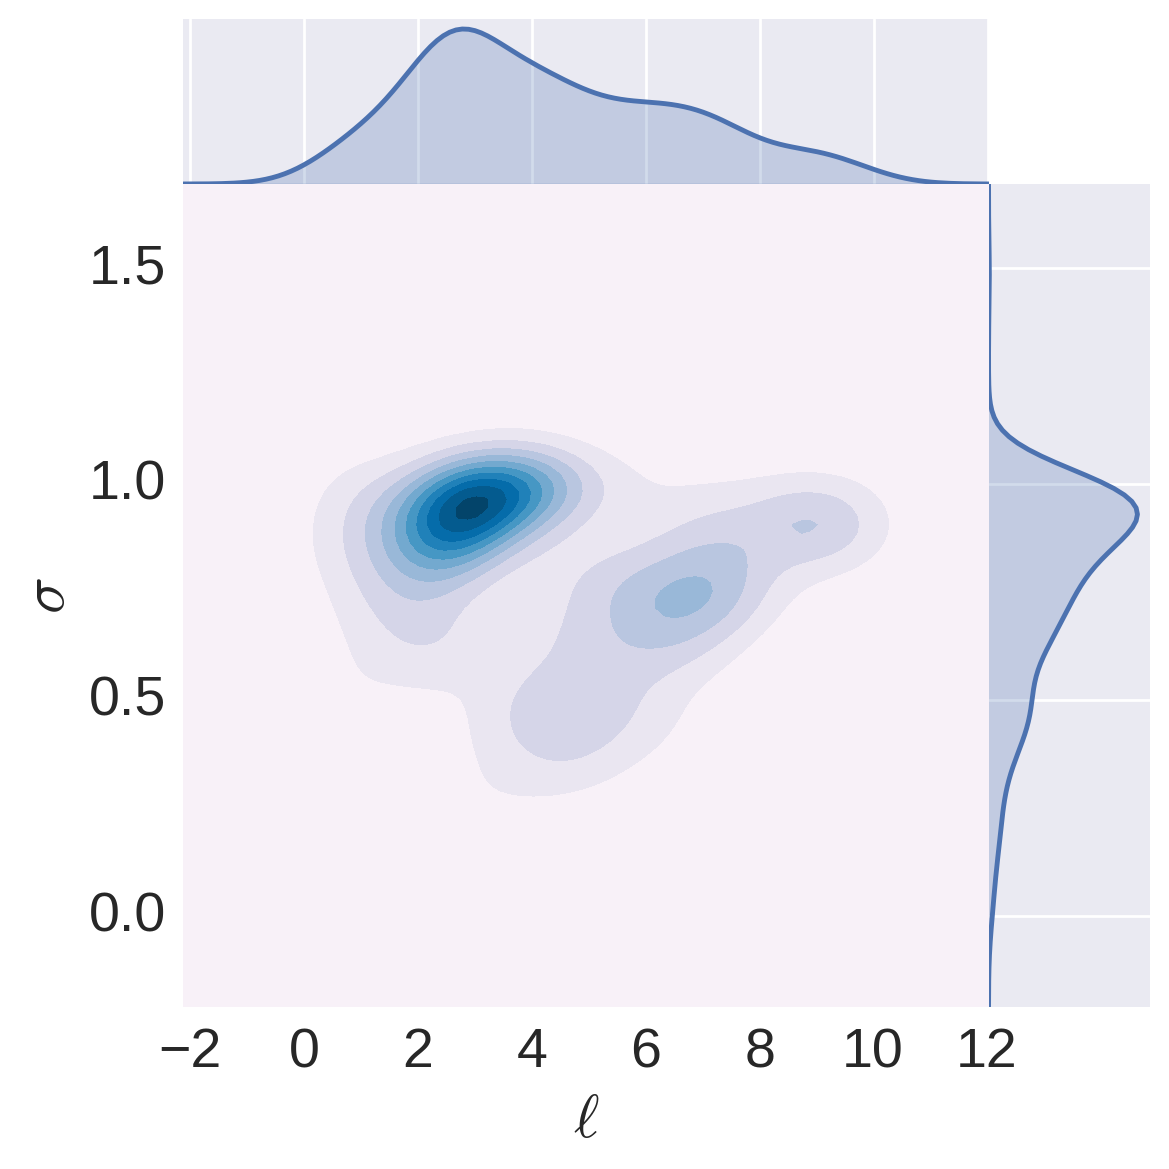
\includegraphics[height=6.5cm]{figs/neal_contour_l_vs_sigma_s__marginal_after.png}
                \caption{After}
                \label{fig:after))}
        \end{subfigure}
        \caption{Hyper-parameter inference on the parameter of the noise kernel. We show a 100 samples drawn from the distribution on $\sigma$. One can clearly recognise the shift from the uniform prior $\mathcal{U}(0,5)$ to a double peak distribution around the two modes - normal and outlier.}\label{fig:inference}
\end{figure}

\subsubsection{Broader applicability of \gpmem}\label{sec:gpmem-broader}

More generally, \gpmem\ is relevant not just when a data set is available, but also whenever we have at hand a function $f_\restr$ which is expensive or impractical to evaluate many times.
\gpmem\ allows us to model $f_\restr$ with a GP-based emulator $f_\emu$, and also to use $f_\emu$ during the learning process to choose, in an online manner, an effective set of probe points $\{x_i\}$ on which to use our few evaluations of $f_\restr$.
This idea is illustrated in detail in Section \ref{sec:bayesopt}.
Before doing this, we will illustrate another benefit of having a probabilistic programming apparatus for GP modelling: the linguistically unified treatment of inference over structure and inference over parameters.
This unification makes interleaved joint inference over structure and parameters very natural, and allows us to give a short, elegant description of what it means to ``learn the covariance function,'' both in prose and in code.
Furthermore, the example in Section \ref{sec:structurelearning} below recovers the performance of current state-of-the-art GP-based models.



\subsection{Structure Learning}\label{sec:structurelearning}
The space of possible kernel composition is infinite. Combining inference over this space with the problem of finding a good parameterization that could potentially explain the observed data best poses a hard problem. The natural language interpretation of the meaning of a kernel and it's composition renders this a problem of symbolic computation. Duvenaud and colleagues note that a sum of kernels can be interpreted as logical OR operations and kernel multiplication as logical AND~\citeyearpar{duvenaud2013structure}. This is due to the kernel rendering two points similar if $k_1$ OR $k_2$ outputs a high value in the case of a sum. Respectively, multiplication of two kernels results in high values only if $k_1$ AND $k_2$ have high values (see Fig. \ref{fig:composite} examplifies how to interpret global vs. local aspects and its symbolic analog respectively). 
In the following, we will refer to covariance functions that are not composite as base covariance functions.

\begin{figure}
\centering

\usetikzlibrary{arrows}


\begin{tikzpicture}[->,>=stealth',level/.style={sibling distance = 5cm/#1,
  level distance = 4.5cm}] 
\node [   align=left] {
                   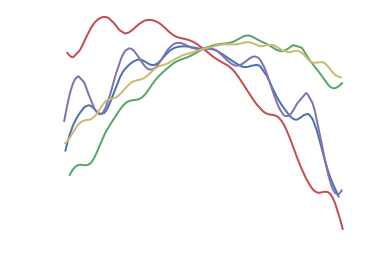
\includegraphics[width=.33\textwidth]{figs/gpSamples/main.png}
\\
SE $\times$ LIN $+$ PER $\times$ LIN $+$  RQ $\times$ LIN}
      child{ node [  align=center]{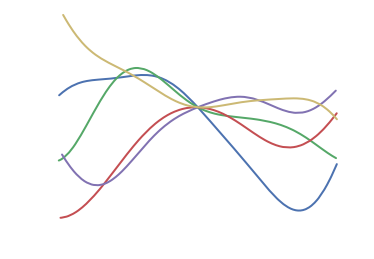
\includegraphics[width=.33\textwidth]{figs/gpSamples/selin.png}\\ SE $\times$ LIN} 
	      child{ node [   align=center] {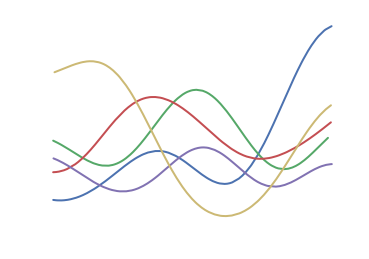
\includegraphics[width=.2\textwidth]{figs/gpSamples/se.png}\\ SE}}
	      child{ node [   align=center] {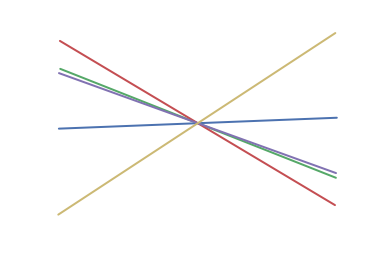
\includegraphics[width=.2\textwidth]{figs/gpSamples/lin.png}\\ LIN }}                            
      }
        child{ node [  align=center]{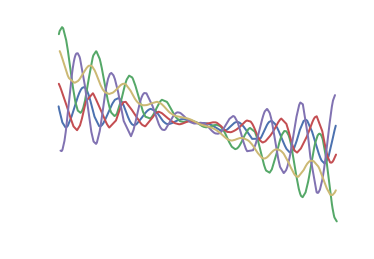
\includegraphics[width=.33\textwidth]{figs/gpSamples/perlin.png}\\ PER $\times$ LIN} 
            child{ node [   align=center] {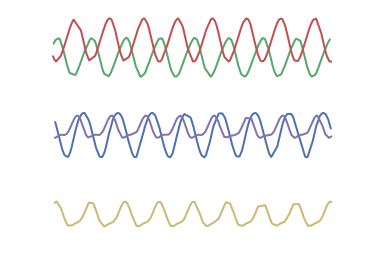
\includegraphics[width=.2\textwidth]{figs/gpSamples/per.png}\\ PER}} 
            child{ node [   align=center] {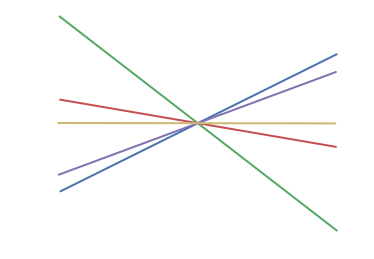
\includegraphics[width=.2\textwidth]{figs/gpSamples/lin2.png}\\ LIN}}
		}
      child{ node [  align=center]{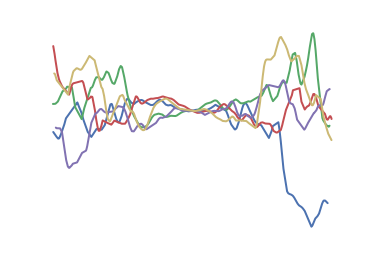
\includegraphics[width=.33\textwidth]{figs/gpSamples/rqlin.png}\\ RQ $\times$ LIN} 
            child{ node [   align=center] {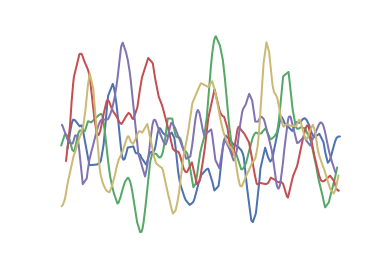
\includegraphics[width=.2\textwidth]{figs/gpSamples/rq.png}\\ RQ}}
            child{ node [   align=center] {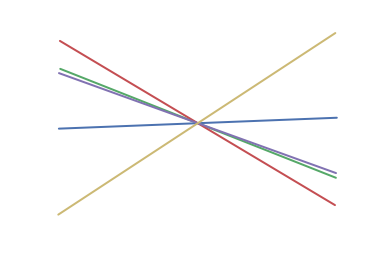
\includegraphics[width=.2\textwidth]{figs/gpSamples/lin.png}\\ LIN}}
		}
; 
\end{tikzpicture}

\caption{Composition of covariance function parsed using the example SE $\times$ LIN $+$ PER $\times$ LIN $+$  RQ $\times$ LIN}\label{fig:composite}
\end{figure}


Knowledge about the composite nature of covariance functions is not new, however, until recently, the choice and the composition of covariance functions were done ad-hoc. The Automated Statistician Project came up with an approximate search over the possible space of kernel structures~\citep{duvenaud2013structure,lloyd2014automatic}. However, a fully Bayesian treatment of this was not done before.
The case where the covariance structure is not given is even more interesting. Our probabilistic programming based MCMC framework approximates the following intractable integrals of the expectation for the prediction:
\begin{equation}
\mathbb{E}[y^* \mid x^*,\mathbf{D},\mathbf{K}] =\iint f(x^*,\bm{\theta},\mathbf{K})\,P(\bm{\theta} \mid \mathbf{D,\mathbf{K}})\,P(\mathbf{K}|\bm{\Omega},s,n) \; \mathbf{d} \bm{\theta} \mathbf{d} \mathbf{K}.  
\end{equation}
This is done by sampling from the posterior probability distribution of the hyper-parameters and the possible kernel:
\begin{equation}
y^* \approx \frac{1}{T} \sum^T_{t=1} f(x^* | \bm{\theta}^{(t)},\mathbf{K}^{(t)}). 
\end{equation}


In order to provide the sampling of the kernel, we introduce a stochastic process to the SP that simulates the grammar for algebraic expressions of covariance function algebra:
\begin{equation}
\mathbf{K}^{(t)} \sim  P(\mathbf{K} \mid \bm{\Omega},s,n)
\end{equation}
Here, we start with a set of possible kernels and draw a random subset. For this subset of size $n$, we sample a set of possible operators that operate on the base kernels. 

The marginal probability of a kernel structure which allows us to sample  is characterized by the probability of a uniformly chosen subset of the set of $n$ possible covariance functions times the probability of sampling a global or a local structure which is given by a binomial distribution: 

\begin{equation}
P(\mathbf{K} \mid \bm{\Omega},s,n) = P(\bm{\Omega} \mid s,n)\times P(s \mid n) \times P(n),
\end{equation}
with
\begin{equation}
P(\bm{\Omega} \mid s,n)= {n \choose r}  p_{+\times}^k (1 - p_{+\times})^{n-k}
\end{equation}
and
\begin{equation}
\label{eq:subsets}
P(s \mid n) = \frac{n!}{ \mid s \mid !}
\end{equation}
where $P(n)$ is a prior on the number of base kernels used which can sample from a discrete uniform distribution. This will strongly prefer simple covariance structures with few base kernels since individual base kernels are more likely to be sampled in this case due to (\ref{eq:subsets}). Alternatively, we can approximate a uniform prior over structures by weighting $P(n)$ towards higher numbers. It is possible to also assign a prior for the probability to sample global or local structures, however, we have assigned complete uncertainty to this with the probability of a flip $p = 0.5$.



Many equivalent covariance structures can be sampled due to covariance function algebra and equivalent representations with different parameterization~\citep{lloyd2014automatic}. Certain covariance functions can differ in terms of the hyper-parameterization but can be absorbed into a single covariance function with a different parameterization. To inspect the posterior of these equivalent structures we convert each kernel expression into a sum of products and subsequently simplify. Rules for this simplification can be found in appendix B.


For reproducing results from the Automated Statistician Project in a Bayesian fashion we first define a prior on the hypothesis space. Note that, as in the implementation of the Automated Statistician, we upper-bound the complexity of the space of covariance functions we want to explore. We also put vague priors on hyper-parameters.

\begin{minipage}{\linewidth}
\small
\belowcaptionskip=-10pt
\begin{lstlisting}[frame=single,mathescape,label=alg:structureVent,basicstyle=\selectfont\ttfamily]
// GRAMMAR FOR KERNEL STRUCTURE
assume base_kernels = list(se, wn, lin, per, rq) // defined as above

// prior on the number of kernels
assume p_number_k = tag('number_kernels, uniform_structure(n))
assume s = tag('choice_subset, subset(base_kernels, p_number_k))

assume cov_compo = proc(l) {
  // kernel composition
  if (size(l) <= 1)
  then { first(l) }
  else { if (flip()) then { add_funcs(first(l), cov_compo(rest(l))) }
                     else { mult_funcs(first(l), cov_compo(rest(l))) }
       }
  }
                          
assume K = tag('composit, cov_compo(s))

assume (f_compute f_emu) = gpmem(f_restr, K)
predict mapv(f_compute(get_data_xs)) // probe all data points

// PERFORMING INFERENCE  
infer  repeat(2000, do(
                        mh('number_kernel, one, 1),
                        mh('choice_subset, one, 1),
                        mh('composit, one, 1),
                        mh('hyper, one, 10)))
\end{lstlisting}

\end{minipage}




We defined the space of covariance structures in a way allowing us to reproduce results for covariance function structure learning as in the Automated Statistician. This lead to coherent results, for example for the airline data set describing monthly totals of international airline passengers (\citealp{box2011time}, according to \citealp{duvenaud2013structure}. We will elaborate the result using a sample from the posterior (Fig. \ref{fig:tutorial}). The sample is identical with the highest scoring result reported in previous work using a search-and-score method~\citep{duvenaud2013structure} for the CO$_2$ data set (see \citealp{rasmussen2006gaussian} for a description) and the predictive capability is comparable. However, the components factor in a different way due to different parameterization of the individual base kernels.

\begin{comment}
\begin{figure}
        \centering
        \begin{subfigure}[b]{\textwidth} \centering
                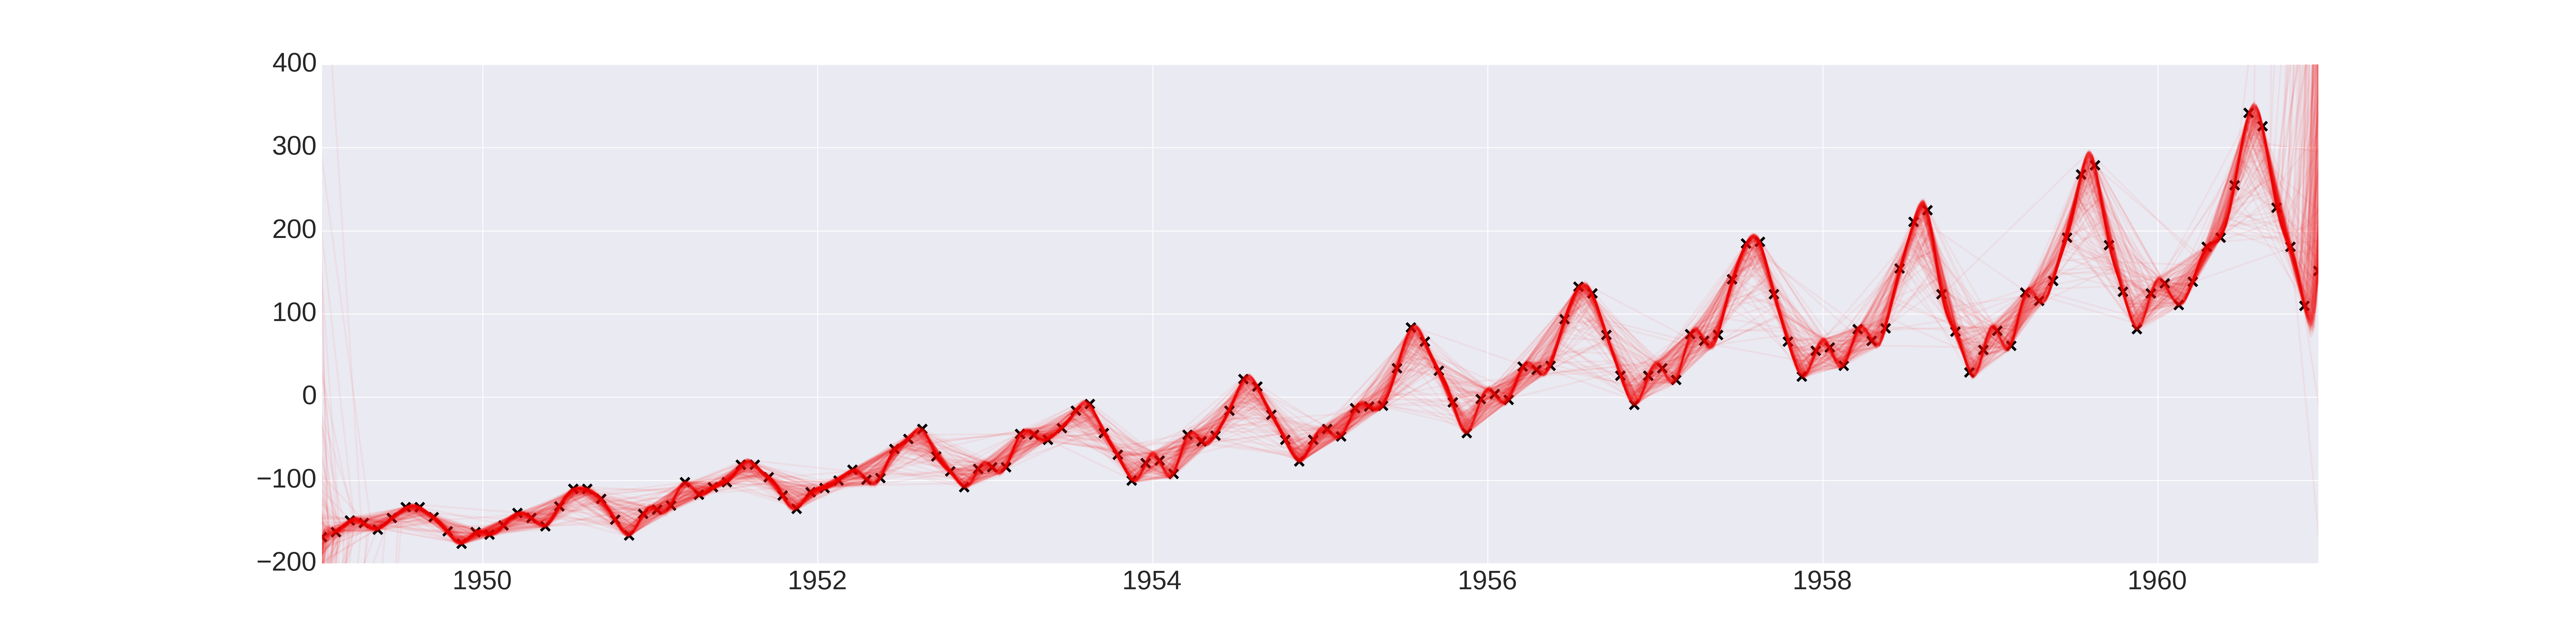
\includegraphics[height=3cm]{figs/airline_tree_3x.png}
                \caption{The predictive posterior using the full grammar structure.}
                \label{fig:airlineBO}
        \end{subfigure}%
        ~ %add desired spacing between images, e. g. ~, \quad, \qquad, \hfill etc.
          %(or a blank line to force the subfigure onto a new line)
          
        \begin{subfigure}[b]{\textwidth} \centering
                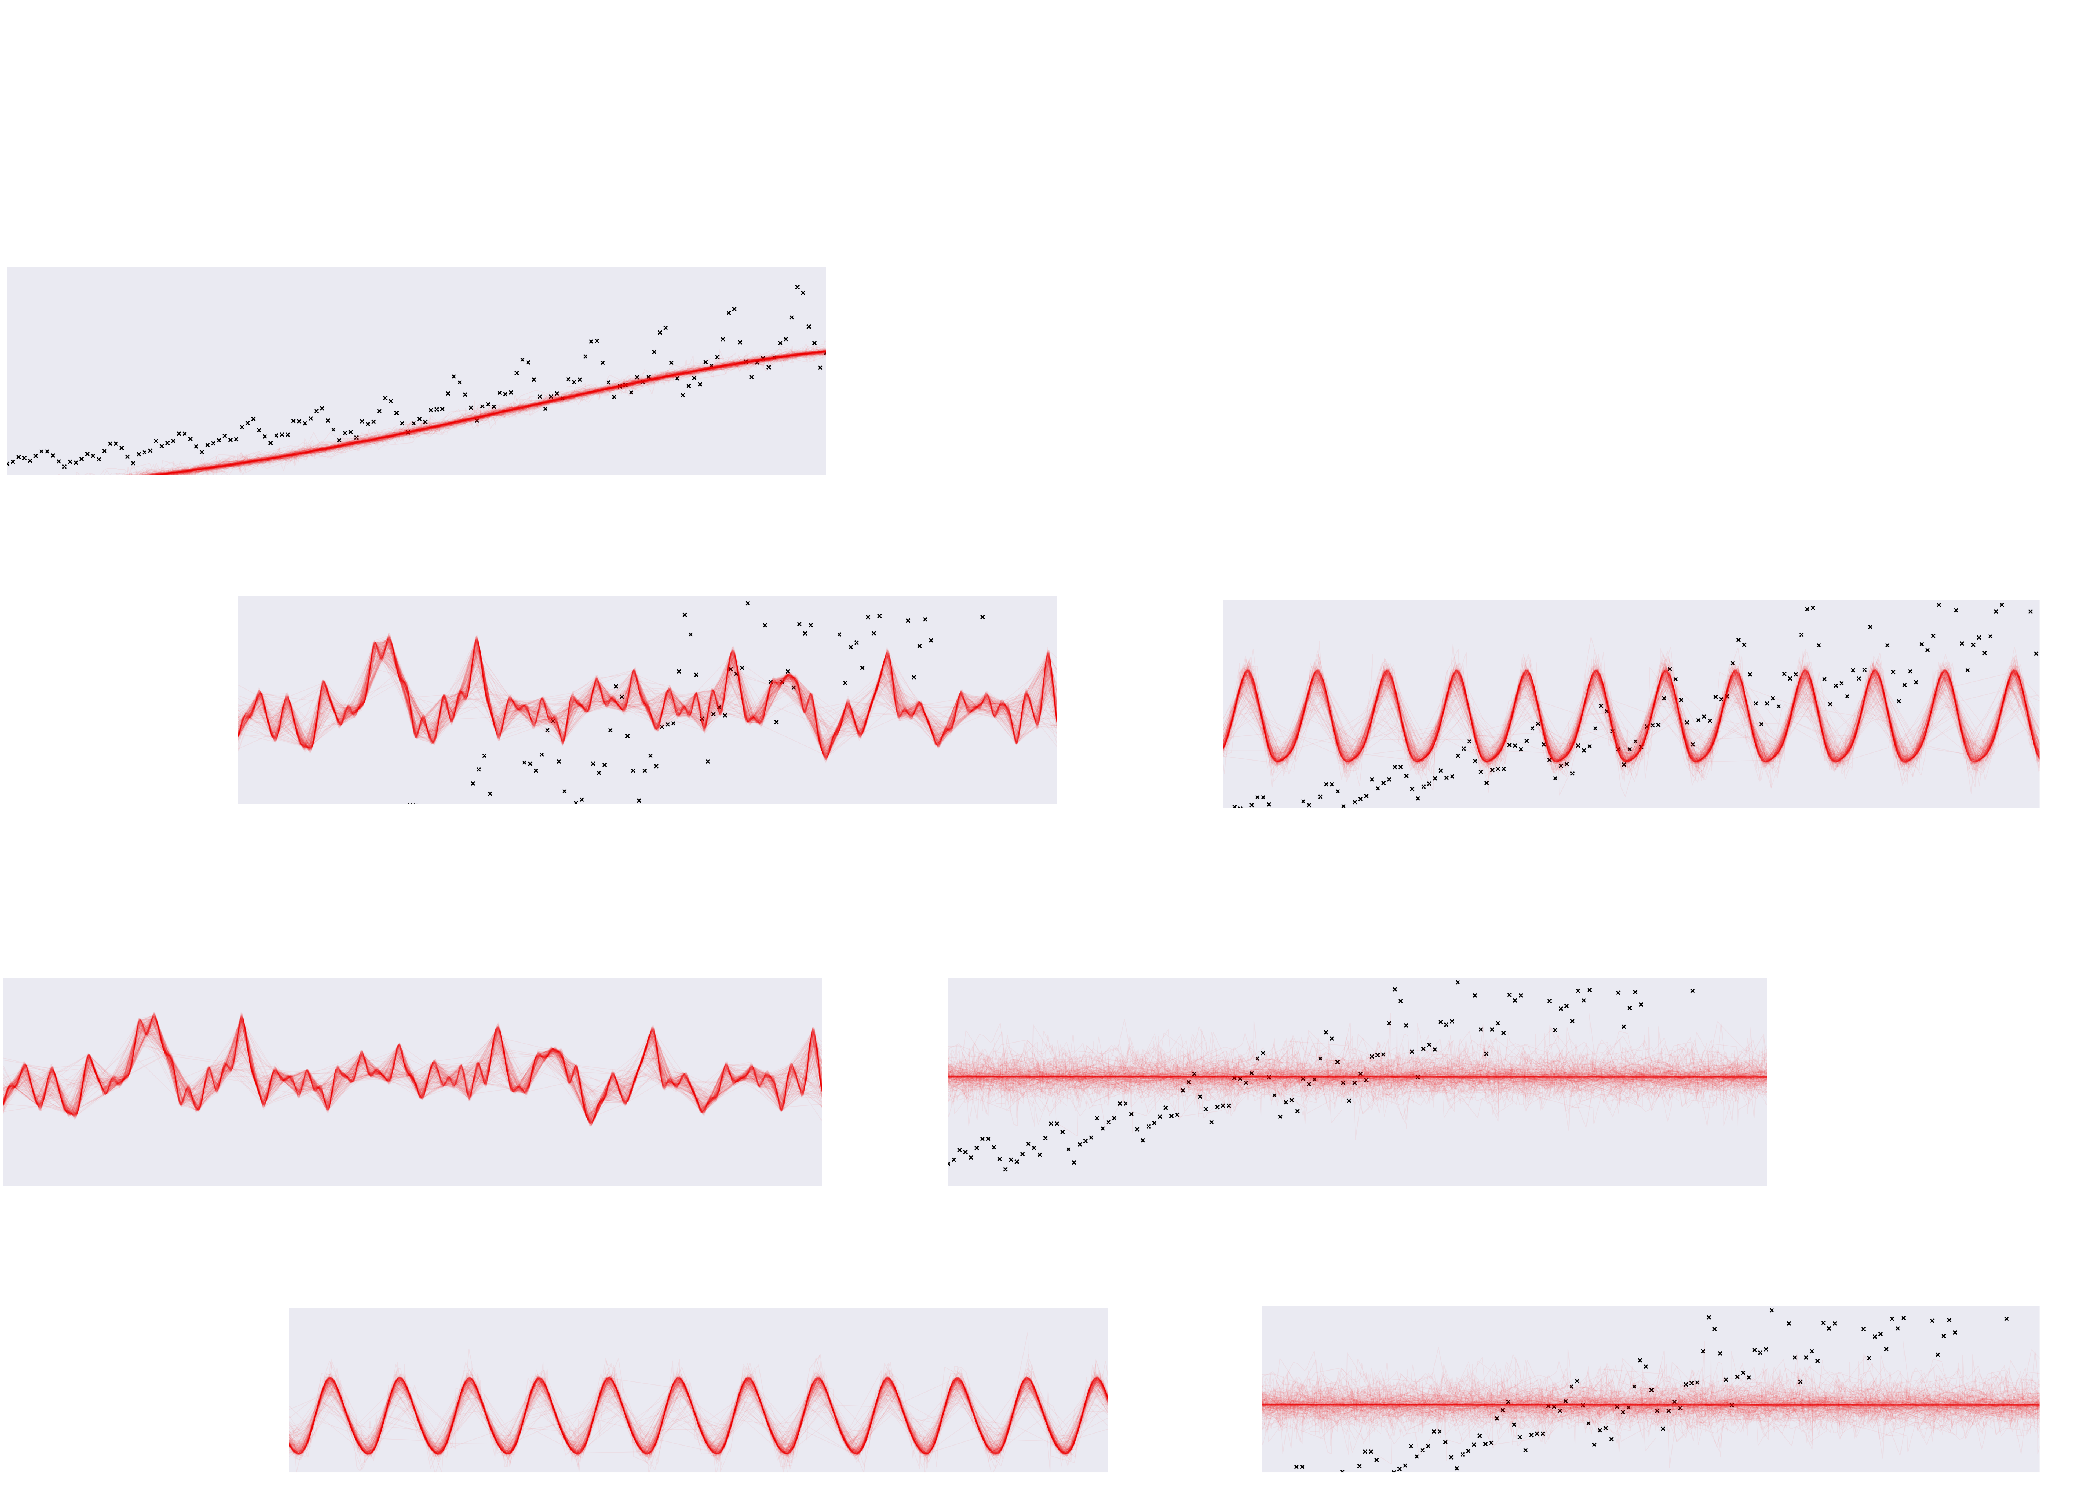
\includegraphics[width=\textwidth]{figs/grammar_tutorial2.png}
                \caption{Compositional Structure}
                \label{fig:AirlineA))}
        \end{subfigure}
        \put(-270,280){SE $\times$ LIN + SE $\times$ LIN (RQ + PER ) $\;\;\; = $} 
        \put(-271,269){\rotatebox{90}{\Large $\Bigg\{$}} 
        \put(-250,267){\vector(-3,-1){30}}
        \put(-220,230){{\Large $+\;\;\;\;\;\;$}SE $\times$ (LIN $\times$ RQ + LIN $\times$ PER) $\;\;\; = $} 
        \put(-395,165){SE {\Large $\times$ \bigg(}} 
        \put(-5,165){\Large \bigg)} 
        \put(-185,165){\Large $+$} 
        \put(-230,146){\vector(0,-1){10}}
        \put(-20,146){\line(0,-1){78}}
        \put(-20,68){\vector(-1,0){150}}
        \put(-251,130){\rotatebox{270}{\Large $\Bigg\{$}} 
        \put(-235,95){\Large $\times$} 
        \put(-191,67){\rotatebox{270}{\Large $\Bigg\{$}} 
        \put(-175,33){\Large $\times$} 
        \caption{a) We see the predictive posterior as a result 1000 nested MH steps on the airline data set. b) depicts a decomposition of this posterior for the structures sampled by Venture. RQ is the rational quadratic covariance function. The first line shows the global trend and denotes the rest of the structure that is shown above. In the second line, the see the periodic component on the right hand side. The left hand side denotes short term deviations both multiplied by a smoothing kernel. The third and fourth lines denote how we reach the second line: both periodic and rational quadratic covariance functions are multiplied by a linear covariance function with slope zero.}\label{fig:tutorial}
\end{figure}
\end{comment}

\begin{figure}
        \centering
        \begin{subfigure}[b]{\textwidth} \centering
                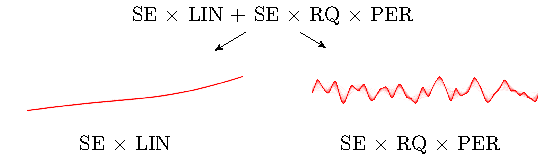
\includegraphics[width=\textwidth]{figs/airline_struct_1.pdf}\caption{}
        \end{subfigure}\\
	\begin{subfigure}[b]{\textwidth} \centering
                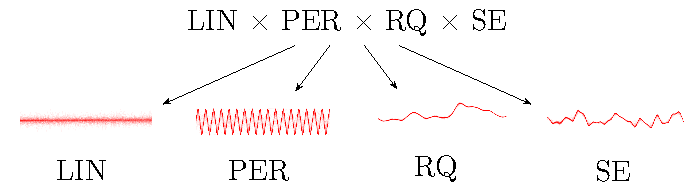
\includegraphics[width=0.9\textwidth]{figs/airline_struct_2.pdf}\caption{}
        \end{subfigure}%
        \caption{(a) most frequent sample drawn from the posterior on structure. We have found two global components. First, A smooth trend (LINxSE) with a non-linear increasing slope. Second, a periodic component with increasing variation and noise. (b) second most frequent sample drawn from the posterior on structure. We found one global component. It is comprised of local changes that are periodic and with changing variation.}\label{fig:posterior_twosamples}
\end{figure}
We further investigated the quality of our stochastic processes by running a leave one out cross-validation to gain confidence on the posterior. This resulted in 545 independent runs of the Markov chain that produced a coherent posterior: our Bayesian interpretation of GP structure and GPs produced a posterior of structures that is in line with previous results on this data set (~\citealp*{duvenaud2013structure}; see Fig. \ref{fig:structureCo2}).

We ran similar evaluation on the airline data set resulting in a similar structure to what was previously reporte (Fig. \ref{fig:structureAir}, residuals and log-score along the Markov chain see Fig. \ref{fig:reslog}).

We found the final sample of multiple runs to be most informative. This kind of Markov Chain seems to produce samples that are highly auto-correlated.
\begin{comment}
\begin{figure}
\centering
    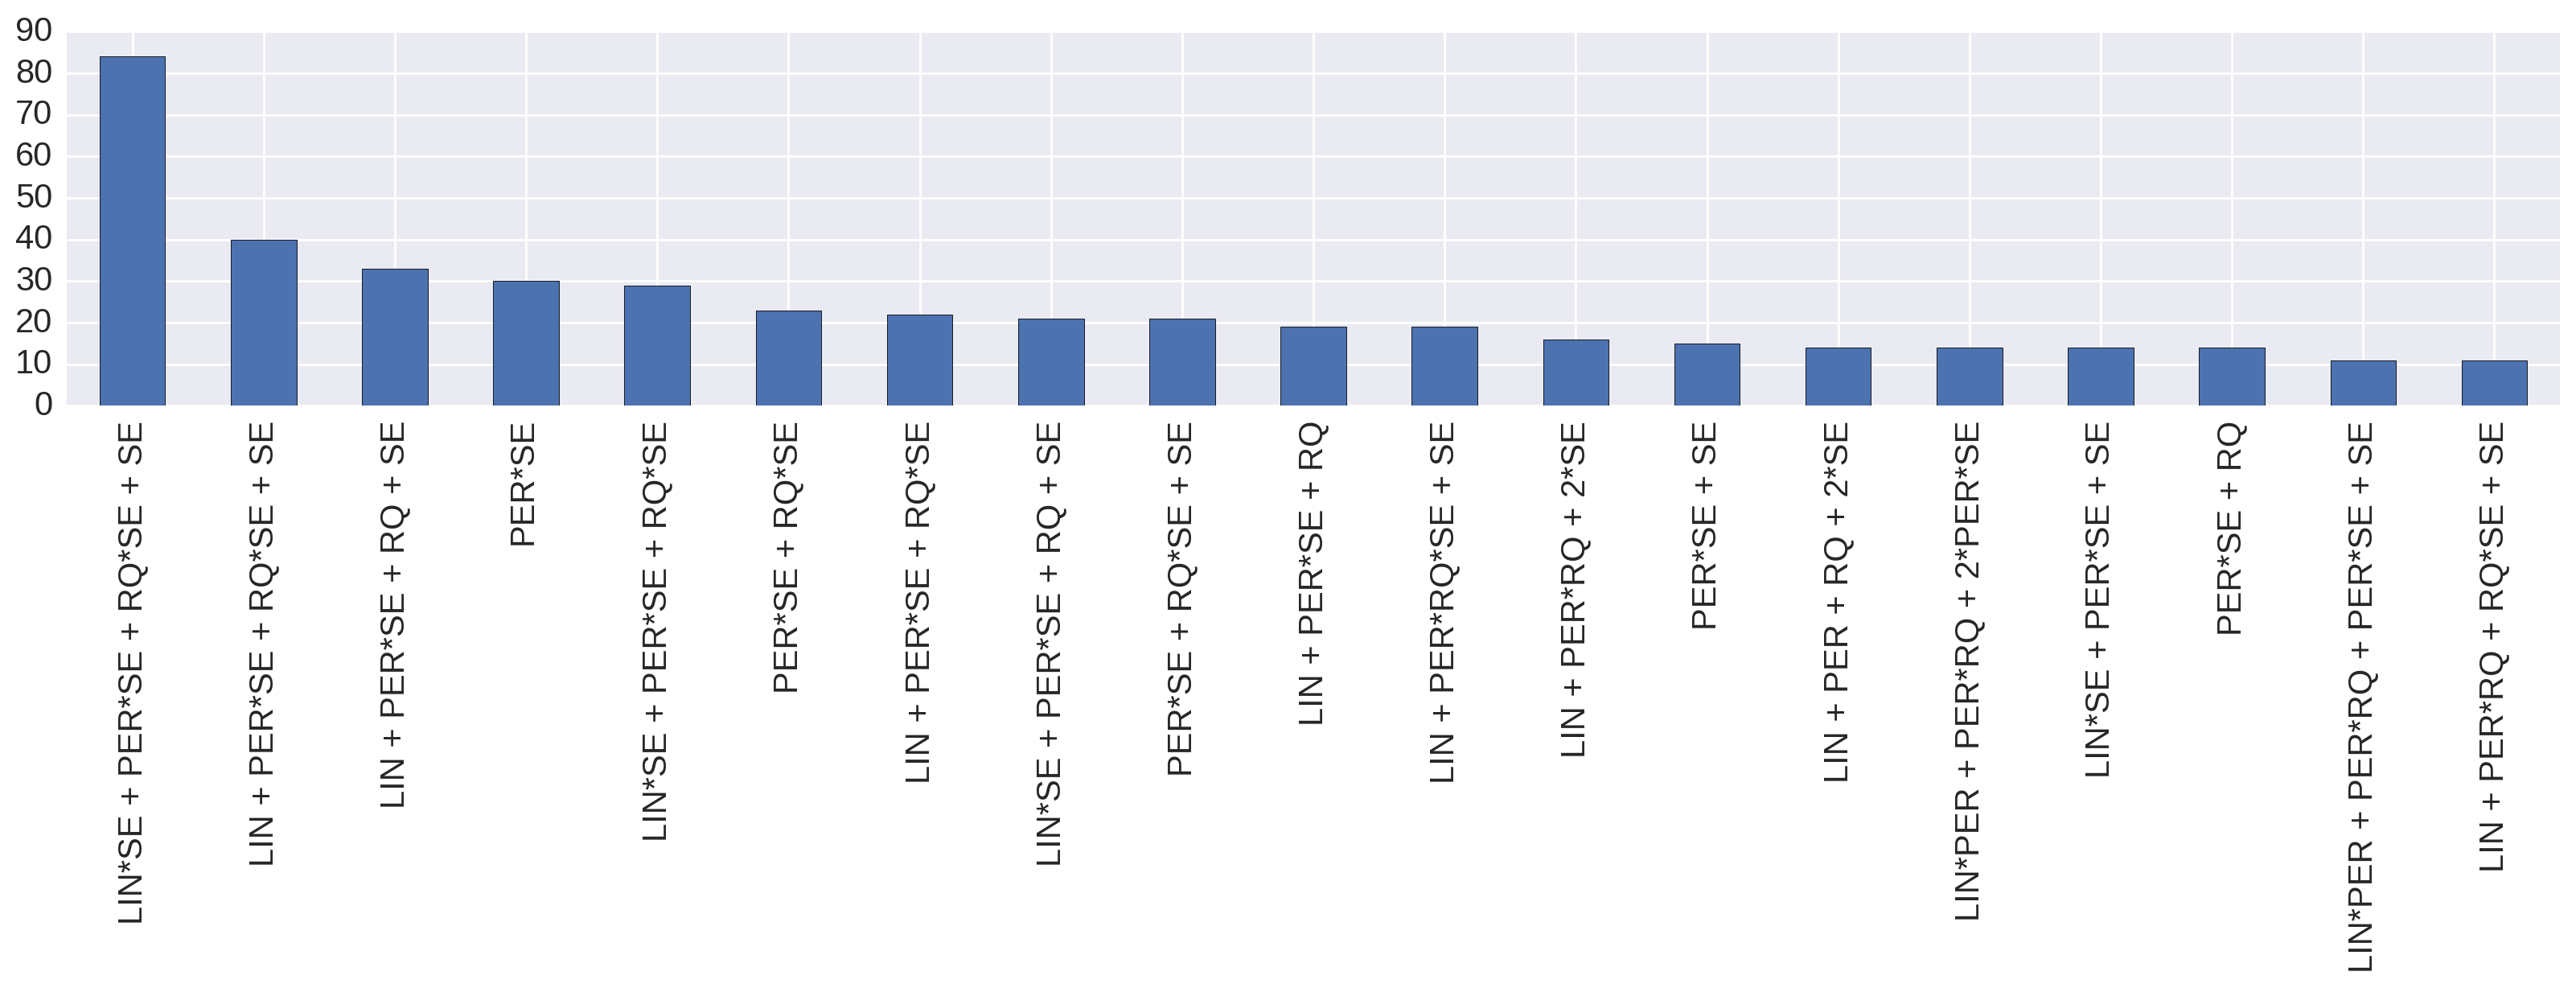
\includegraphics[width=\textwidth]{figs/structureCo2b.png}
    \caption{Posterior on structure of the CO2 data. We have cut the tail of the distribution for space reasons since the number of possible structures is large. We see the final sample of the each of the 545 chains with 2000 nested steps each. Note that \citet{duvenaud2013structure} report LIN $\times$ SE $+$ PER $\times$ SE $+$ RQ $\times$ SE.}\label{fig:structureCo2}
\end{figure}

\begin{figure}
\centering
    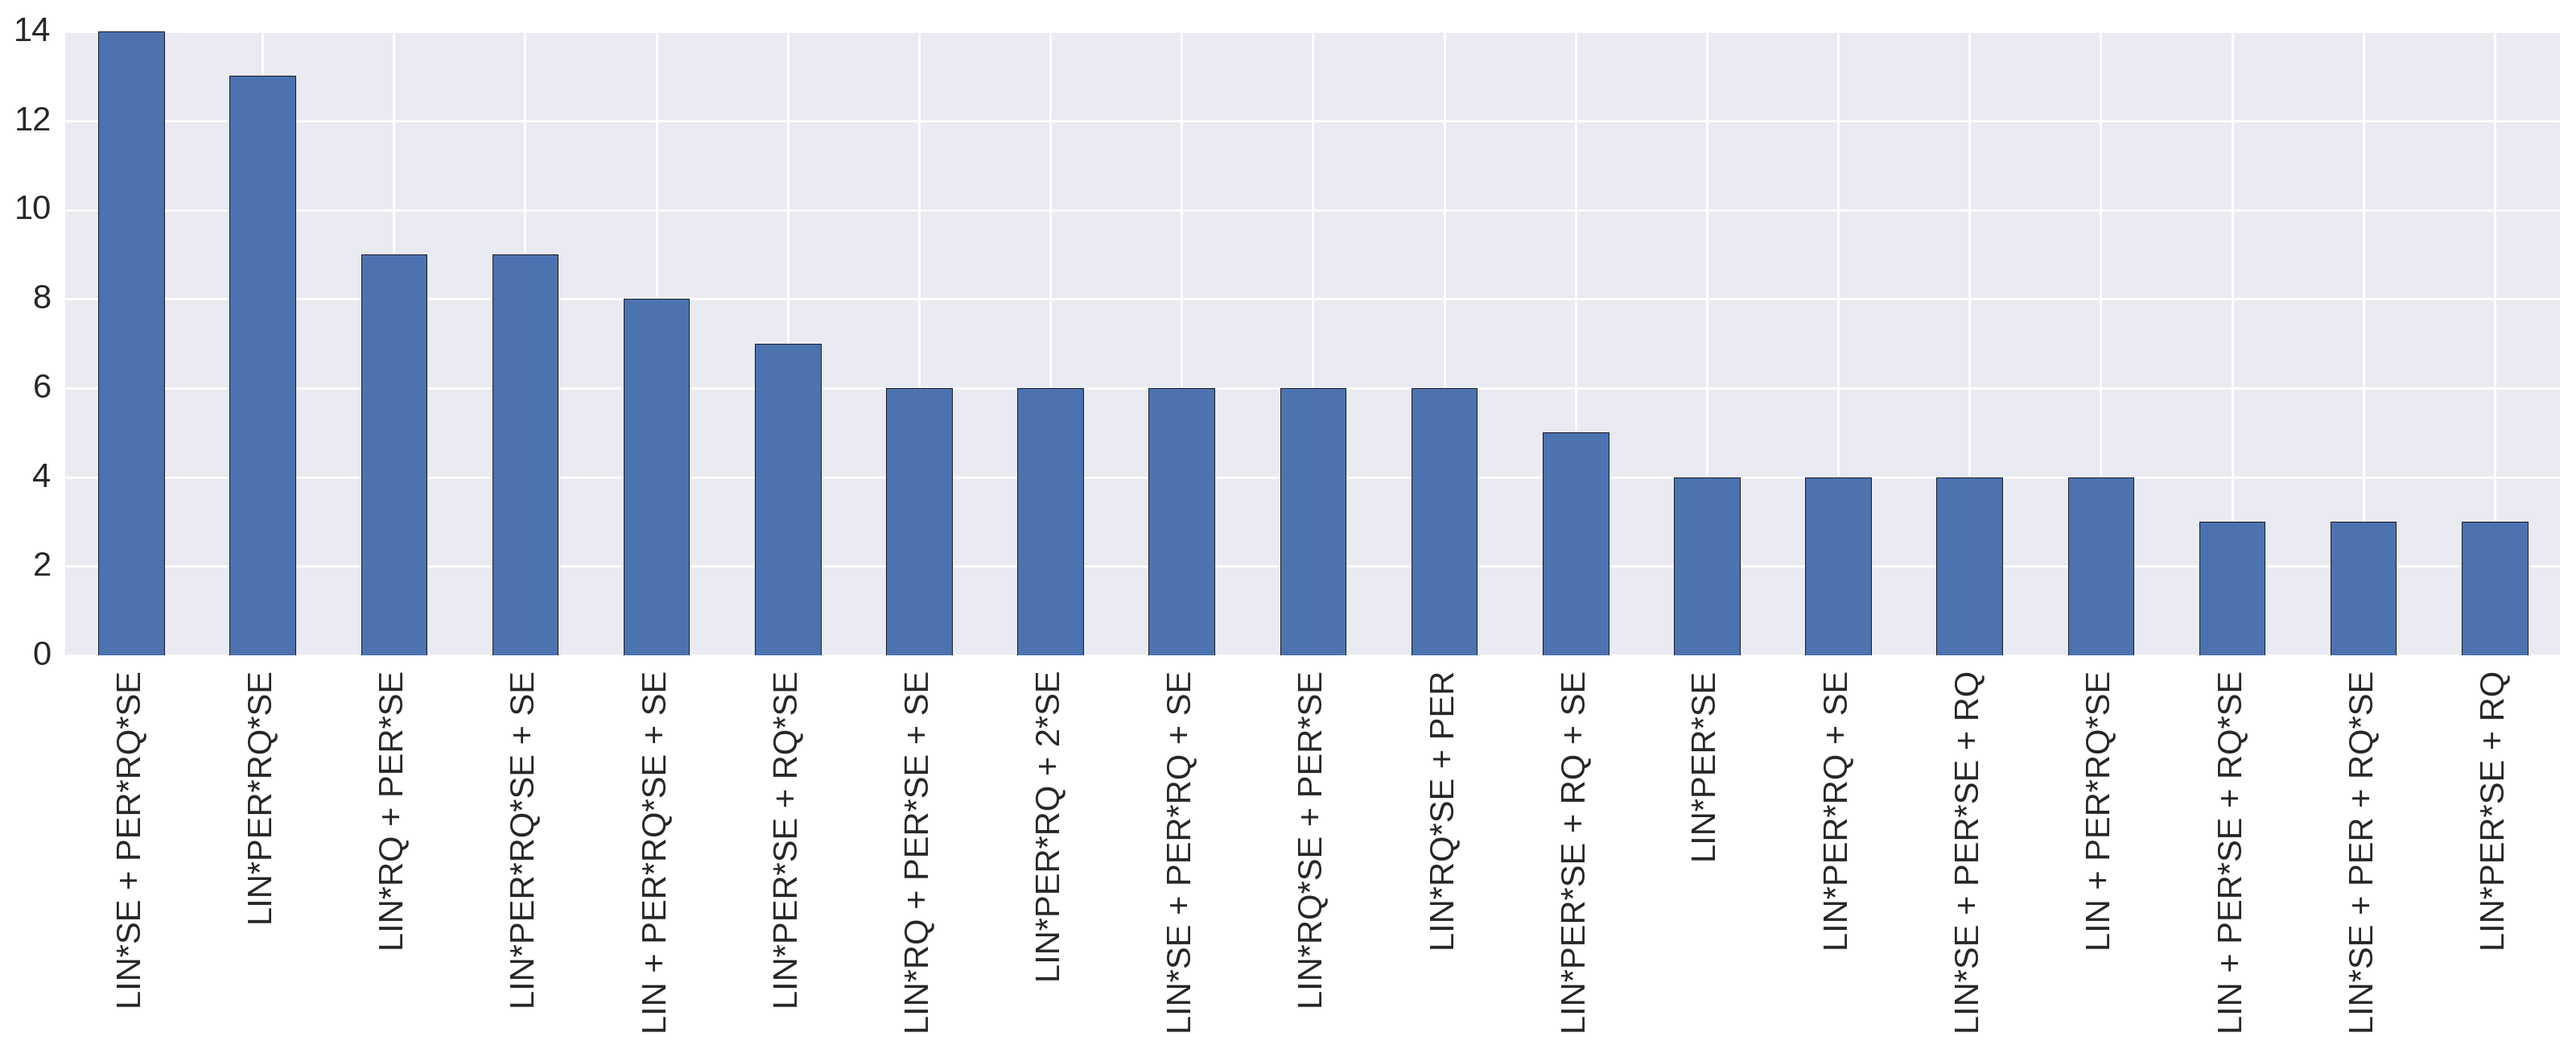
\includegraphics[width=\textwidth]{figs/structureAirlinec.png}
    \caption{Posterior on structure of airline data set. We have cut the tail of the distribution for space reasons since the number of possible structures is large. We see the final sample of the each of the 144 chains with 2000 nested steps each. Note that \citet{duvenaud2013structure} report LIN $\times$ SE $+$ (PER  + RQ) $\times$ SE $\times$ LIN}\label{fig:structureAir}
\end{figure}


\begin{figure}
        \centering
        \begin{subfigure}[b]{0.5\textwidth} \centering
                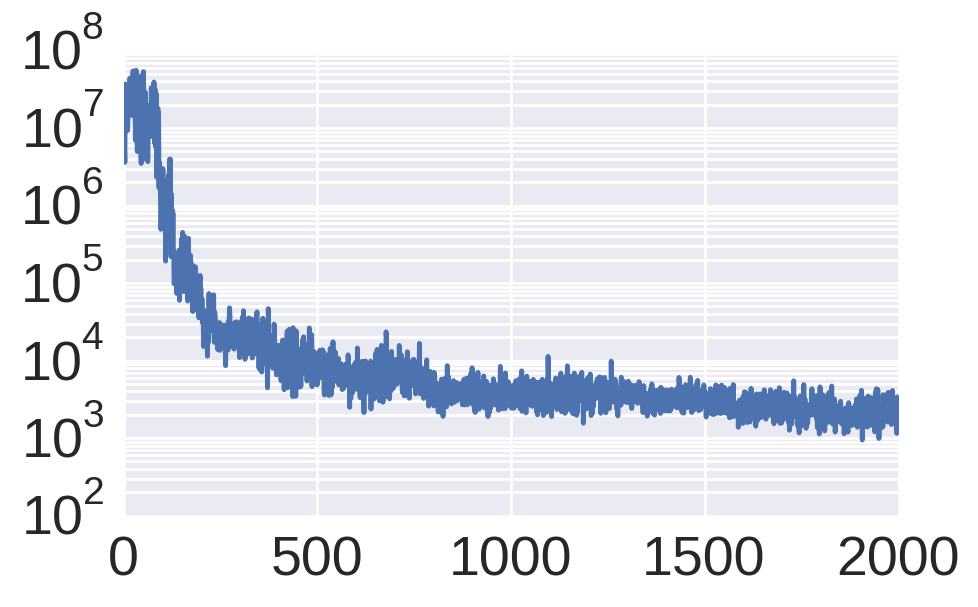
\includegraphics[height=4.5cm]{figs/structureAirline_res_c.png}
                \caption{Residuals}
                \label{fig:res}
        \end{subfigure}%
        ~ %add desired spacing between images, e. g. ~, \quad, \qquad, \hfill etc.
          %(or a blank line to force the subfigure onto a new line)
        \begin{subfigure}[b]{0.5\textwidth} \centering
                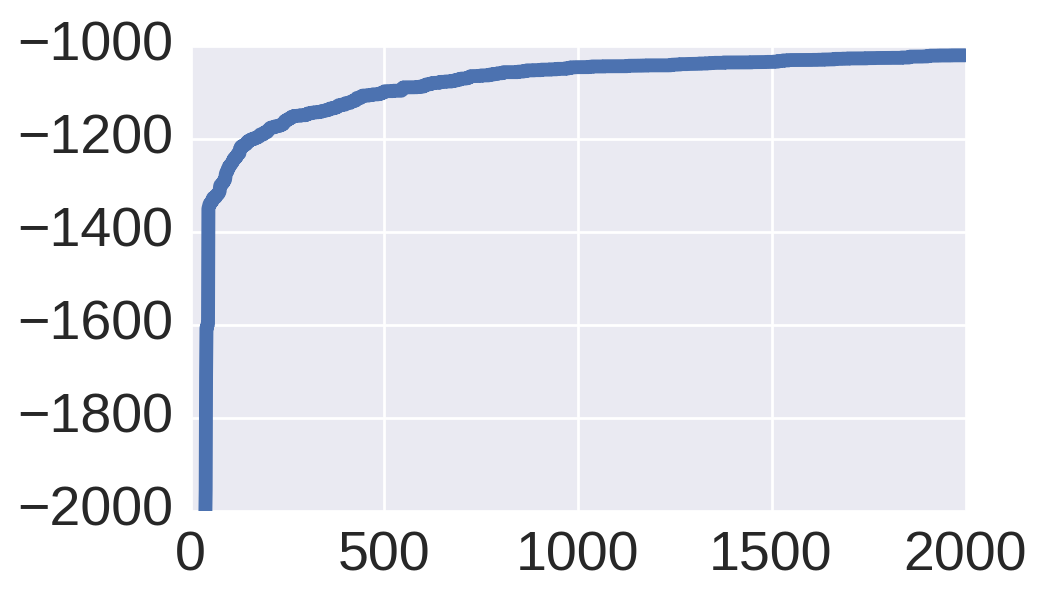
\includegraphics[height=4.5cm]{figs/structureAirline_log_c.png}
                \caption{Log Likelihood}
                \label{fig:log))}
        \end{subfigure}
        \caption{2000 steps along the Markov Chain.}\label{fig:reslog}
\end{figure}
\end{comment}

Given two additive components $\mathbf{K} = \mathbf{K_a} + \mathbf{K_b}$, one can compute the margninal of a global component of a composite kernel structure~\citep{benavoli2015gaussian} with a gaussian posterior $\mathcal{N}(f_a \mid \hat{\mu}_a,\hat{\mathbf{K}}_a)$  where:

\begin{equation}
\label{eq:marginalComponentMean}
\hat{\bm\mu}_a   = \mathbf{K_a}(\xbf,\xbf^*)\, \mathbf{K}(\xbf^*,\xbf^*)^{-1}\, \ybf
\end{equation}
and covariance matrix
\begin{equation}
\label{eq:marginalComponentCovariance}
\hat{\mathbf{K}}_a =   \mathbf{K_a}(\xbf,\xbf) -  \mathbf{K_a}(\xbf,\xbf^*)\mathbf{K}(\xbf^*,\xbf^*)^{-1} \mathbf{K_a}(\xbf^*,\xbf).
\end{equation}

\FloatBarrier
\section{Bayesian Optimization}\label{sec:bayesopt}
Bayesian optimization casts the problem of finding the global maximum of an unknown function as a hierarchical decision problem~\citep{ghahramani2015probabilistic}.
Evaluating the actual function may be very expensive, either in computation time or in some other resource.
For one example, when searching for the best configuration for the learning algorithm of a large convolutional neural network, a large amount of computational work is required to evaluate a candidate configuration, and the space of possible configurations is high-dimensional.
Another common example, alluded to in Section \ref{sec:gpmem-broader}, is data acquisition: for machine learning problems in which a large body of data is available, it is often desirable to choose the right queries to produce a data set on which learning will be most effective.
In continuous settings, many Bayesian optimization methods employ GPs~\citep[e.g.][]{snoek2012practical}.

We have implemented a version of Thompson sampling using GPs in Venture.
Thompson sampling~\cite{thompson1933likelihood} is a widely-used Bayesian framework for solving exploration-exploitation problems.
Our implementation has two notable features: (i) the ability to search over a broader space of contexts than the parametric families that are typically used, and (ii) the parsimony of the resulting probabilistic program.

\subsection{Thompson sampling framework}
We now lay out the setup of Thompson sampling for Markov decision processes (MDPs).
An agent is to take a sequence of actions $a_1, a_2, \ldots$ from a (possibly infinite) set of possible actions $\Acal$.
After each action, a reward $r \in \R$ is received, according to an unknown conditional distribution $P_\true(r|a)$.
The agent's goal is to maximize the total reward received for all actions.
In Thompson sampling, the Bayesian agent accomplishes this by placing a prior distribution $P(\theta)$ on the possible ``contexts'' $\theta \in \Theta$.
Here a context is a believed model of the conditional distributions $\{P(r|a)\}_{a \in \Acal}$, or at least, a believed statistic of these conditional distributions which is sufficient for deciding an action $a$.
One example of such a sufficient statistic is the conditional mean $V(a|\theta) = \Ebkt{r|a,\theta}$, which can be thought of as a value function.
Thompson sampling thus has the following steps, repeated as long as desired:
\begin{enumerate}
  \item Sample a context $\theta \sim P(\theta)$.
  \item Choose an action $a \in \Acal$ which (approximately) maximizes $V(a|\theta) = \Ebkt{r|a,\theta}$.
  \item\label{itm:Thompson-conditioning}
    Let $r_\true$ be the reward received for action $a$.
    Update the believed distribution on $\theta$, i.e., $P(\theta) \gets P_\rmnew(\theta)$ where $P_\rmnew(\theta) = P\pn{\theta \mvert a \mapsto r_\true}$.
\end{enumerate}
Note that when $\Ebkt{r|a,\theta}$ (under the sampled value of $\theta$ for some points $a$) is far from the true value $\Ebkt[P_\true]{r|a}$, the chosen action $a$ may be far from optimal, but the information gained by probing action $a$ will improve the belief $\theta$.
This amounts to ``exploration.''
When $\Ebkt{r|a,\theta}$ is close to the true value except at points $a$ for which $\Ebkt{r|a,\theta}$ is low, exploration will be less likely to occur, but the chosen actions $a$ will tend to receive high rewards.
This amounts to ``exploitation.''
Roughly speaking, exploration will happen until the context $\theta$ is reasonably sure that the unexplored actions are probably not optimal, at which time the sampler will exploit by choosing actions in regions it knows to have high value.

Typically, when Thompson sampling is implemented, the search over contexts $\theta \in \Theta$ is limited by the choice of representation.
In traditional programming environments, $\theta$ often consists of a few numerical parameters for a family of distributions of a fixed functional form.
With work, a mixture of a few functional forms is possible; but without probabilistic programming machinery, implementing a rich context space $\Theta$ would be an unworkably large technical burden.
In a probabilstic programing language, however, the representation of heterogeneously structured or infinite-dimensional context spaces is quite natural.
Any computable model of the conditional distributions $\br{P(r|a)}_{a \in \Acal}$ can be represented as a stochastic procedure $(\lambda (a) \ldots)$.
Thus, for computational Thompson sampling, the most general context space $\widehat\Theta$ is the space of program texts.
Any other context space $\Theta$ has a natural embedding as a subset of $\widehat\Theta$.

\subsection{Thompson sampling in Venture}
Because Venture supports sampling and inference on (stochastic-)procedure-valued random variables (and the generative models which produce those procedures), Venture can capture arbitrary context spaces as described above.
To demonstrate, we have implemented Thompson sampling in Venture in which the contexts $\theta$ are Gaussian processes over the action space $\Acal = \R$.
That is, $\theta = (\mu, K)$, where the mean $\mu$ is a computable function $\Acal \to \R$ and the covariance $K$ is a computable (symmetric, positive-semidefinite) function $\Acal \times \Acal \to \R$.
This represents a Gaussian process $\br{R_a}_{a \in \Acal}$, where $R_a$ represents the reward for action $a$.
% where for any finite subset $\br{a_i}_{i=1}^{n} \subset \Acal$, the marginal distribution on $\pn{R_{a_i}}$ is Gaussian with mean $\pn{\mu(a_i)}_{i=1}^{n}$ and covariance matrix $\begin{pmatrix} K(a_i,a_j) \end{pmatrix}_{1 \leq i,j \leq n}$.
Computationally, we represent a context not as a pair of infinite lookup tables for $\mu$ and $K$, but as a finite data structure $\theta = (K_\prior, \sigma, \ell, \abf_\past, \rbf_\past)$, where
\begin{itemize}
  \item $K_\prior = K_{\prior,\sigma,\ell}$ is a procedure, with parameters $\sigma,\ell$, to be used as the prior covariance function: $K_\prior(a,a') = \sigma^2 \exp\pn{-\frac{(a-a')^2}{2\ell^2}}$
  \item $\sigma$ and $\ell$ are (hyper)parameters for $K_\prior$
  \item $\abf_\past = \pn{a_i}_{i=1}^{n}$ are the previously probed actions
  \item $\rbf_\past = \pn{r_i}_{i=1}^{n}$ are the corresponding rewards
\end{itemize}
To simplify the treatment, we take prior mean $\mu_\prior \equiv 0$.  The mean and covariance for $\theta$ are then gotten by the usual conditioning formula:
\begin{align*}
  \mu(\abf)
  &= \mu\pn{\abf \mvert \abf_\past, \rbf_\past} \\
  &= K_\prior(\abf, \abf_\past)
     \,K_\prior(\abf_\past, \abf_\past)^{-1}
     \,\rbf_\past \\
  K(\abf, \abf)
  &= K\pn{\abf, \abf \mvert \abf_\past, \rbf_\past} \\
  &= K_\prior(\abf, \abf)
     - K_\prior(\abf, \abf_\past)
       \,K_\prior(\abf_\past, \abf_\past)^{-1}
       \,K_\prior(\abf_\past, \abf).
\end{align*}
Note that even in this simple example, the context space $\Theta$ is not a finite-dimensional parametric family, since the vectors $\abf_\past$ and $\rbf_\past$ grow as more samples are taken.
$\Theta$ is, however, quite easily representable as a computational procedure together with parameters and past samples, as we do in the representation $\theta = (K_\prior, \sigma, \ell, \abf_\past, \rbf_\past)$.

\subsection{Implementation with \gpmem}
As a demonstration, we use Thompson sampling to optimize an unknown function $V(x)$ (the value function) using \gpmem.
(\textbf{TODO} we should not assume $V$ is deterministic, it would be easy enough to make it random or have it give noisy samples.)
We assume $V$ is made available to Venture as a black-box.
The code for optimizing $V$ is given in Listing \ref{alg:bayesopt}.
For step \ref{itm:Thompson-conditioning} of Thompson sampling, the Bayesian update, we not only condition on the new data (the chosen action $a$ and the received reward $r$), but also perform inference on the hyperparameters $\sigma, \ell$ using a Metropolis--Hastings sampler.
These two inference steps take 1 line of code: 0 lines to condition on the new data (as this is done automatically by \gpmem), and 1 line to call Venture's built-in \texttt{MH} operator.
The results are shown in Figure \ref{fig:bayesopt-sequence}.
We can see from the figure that, roughly speaking, each successive probe point $a$ is chosen either because the current model $V_\emu$ thinks it will have a high reward, or because the value of $V_\emu(a)$ has high uncertainty.
In the latter case, probing at $a$ decreases this uncertainty and, due to the smoothing kernel, also decreases the uncertainty at points near $a$.
We thus see that our Thompson sampler simultaneously learns the value function and optimizes it.
\begin{comment}
\begin{minipage}{\linewidth}
\small
\belowcaptionskip=-10pt
\begin{lstlisting}[float,frame=single,caption={
  Code for Bayesian optimization using \gpmem.
  %The procedure \texttt{V\_compute} probes \texttt{V} directly, thus improving the GP model \texttt{V\_emu}.
  %(\texttt{V\_emu\_pointwise} is simply a shortcut for sampling the GP model at a single point; \texttt{V\_emu} is more general, allowing joint samples to be taken at any set of points.)
  In the loop, \texttt{V\_compute} is called to probe the value of \texttt{V} at a new argument.
  The new argument, \texttt{(mc\_argmax V\_emu\_pointwise mc\_sampler)}, is a Monte Carlo estimate of the maximum pointwise sample of \texttt{V\_emu} (itself a stochastic quantity), with the Monte Carlo samples being drawn in this case uniformly between $-20$ and $20$.
  After each new call to \texttt{V\_compute}, the Metropolis--Hastings algorithm is used to perform inference on the hyperparameters of the covariance function in the GP model in light of the new conditioning data.
  Once enough calls to \texttt{V\_compute} have been made (in our case we stopped at 15 calls), we can inspect the full list of probed $(a,r)$ pairs with \texttt{extract\_stats}.
  The answer to our maximization problem is simply the pair having the highest $r$; but our algorithm also learns more potentially useful information.
},mathescape,label=alg:bayesopt]
assume log_sf = tag('hyper, log(uniform_continuous(0, 10)))
assume log_l = tag('hyper, log(uniform_continuous(0, 10)))
assume se = make_squaredexp(log_sf, log_l)
assume blackbox_f = get_bayesopt_blackbox()
assume (f_compute, f_emu) = gpmem(blackbox_f, se)

define get_uniform_candidate = proc(prev_xs) {
  uniform_continuous(-20, 20)
}

define mc_argmax = proc(func, prev_xs) {
  // Monte Carlo estimator for the argmax of func.
  run(do(
    candidate_xs <- mapv(proc(i) {get_uniform_candidate(prev_xs)},
                         linspace(0, 19, 20)),
    candidate_ys <- mapv(func, candidate_xs),
    lookup(candidate_xs, argmax_of_array(candidate_ys))))
}

define emulator_point_sample = proc(x) {
  run(sample(lookup(
    f_emu(array(x)),
    0)))
}

infer repeat(15, do(pass,
     // Phase 2: Call f_compute on the next probe point
     predict f_compute(
                 mc_argmax(emulator_point_sample, '_)),
     // Phase 1: Hyperparameter inference
     mh('hyper, one, 50)))
\end{lstlisting}
\end{minipage}
      
\begin{figure}
\centering
    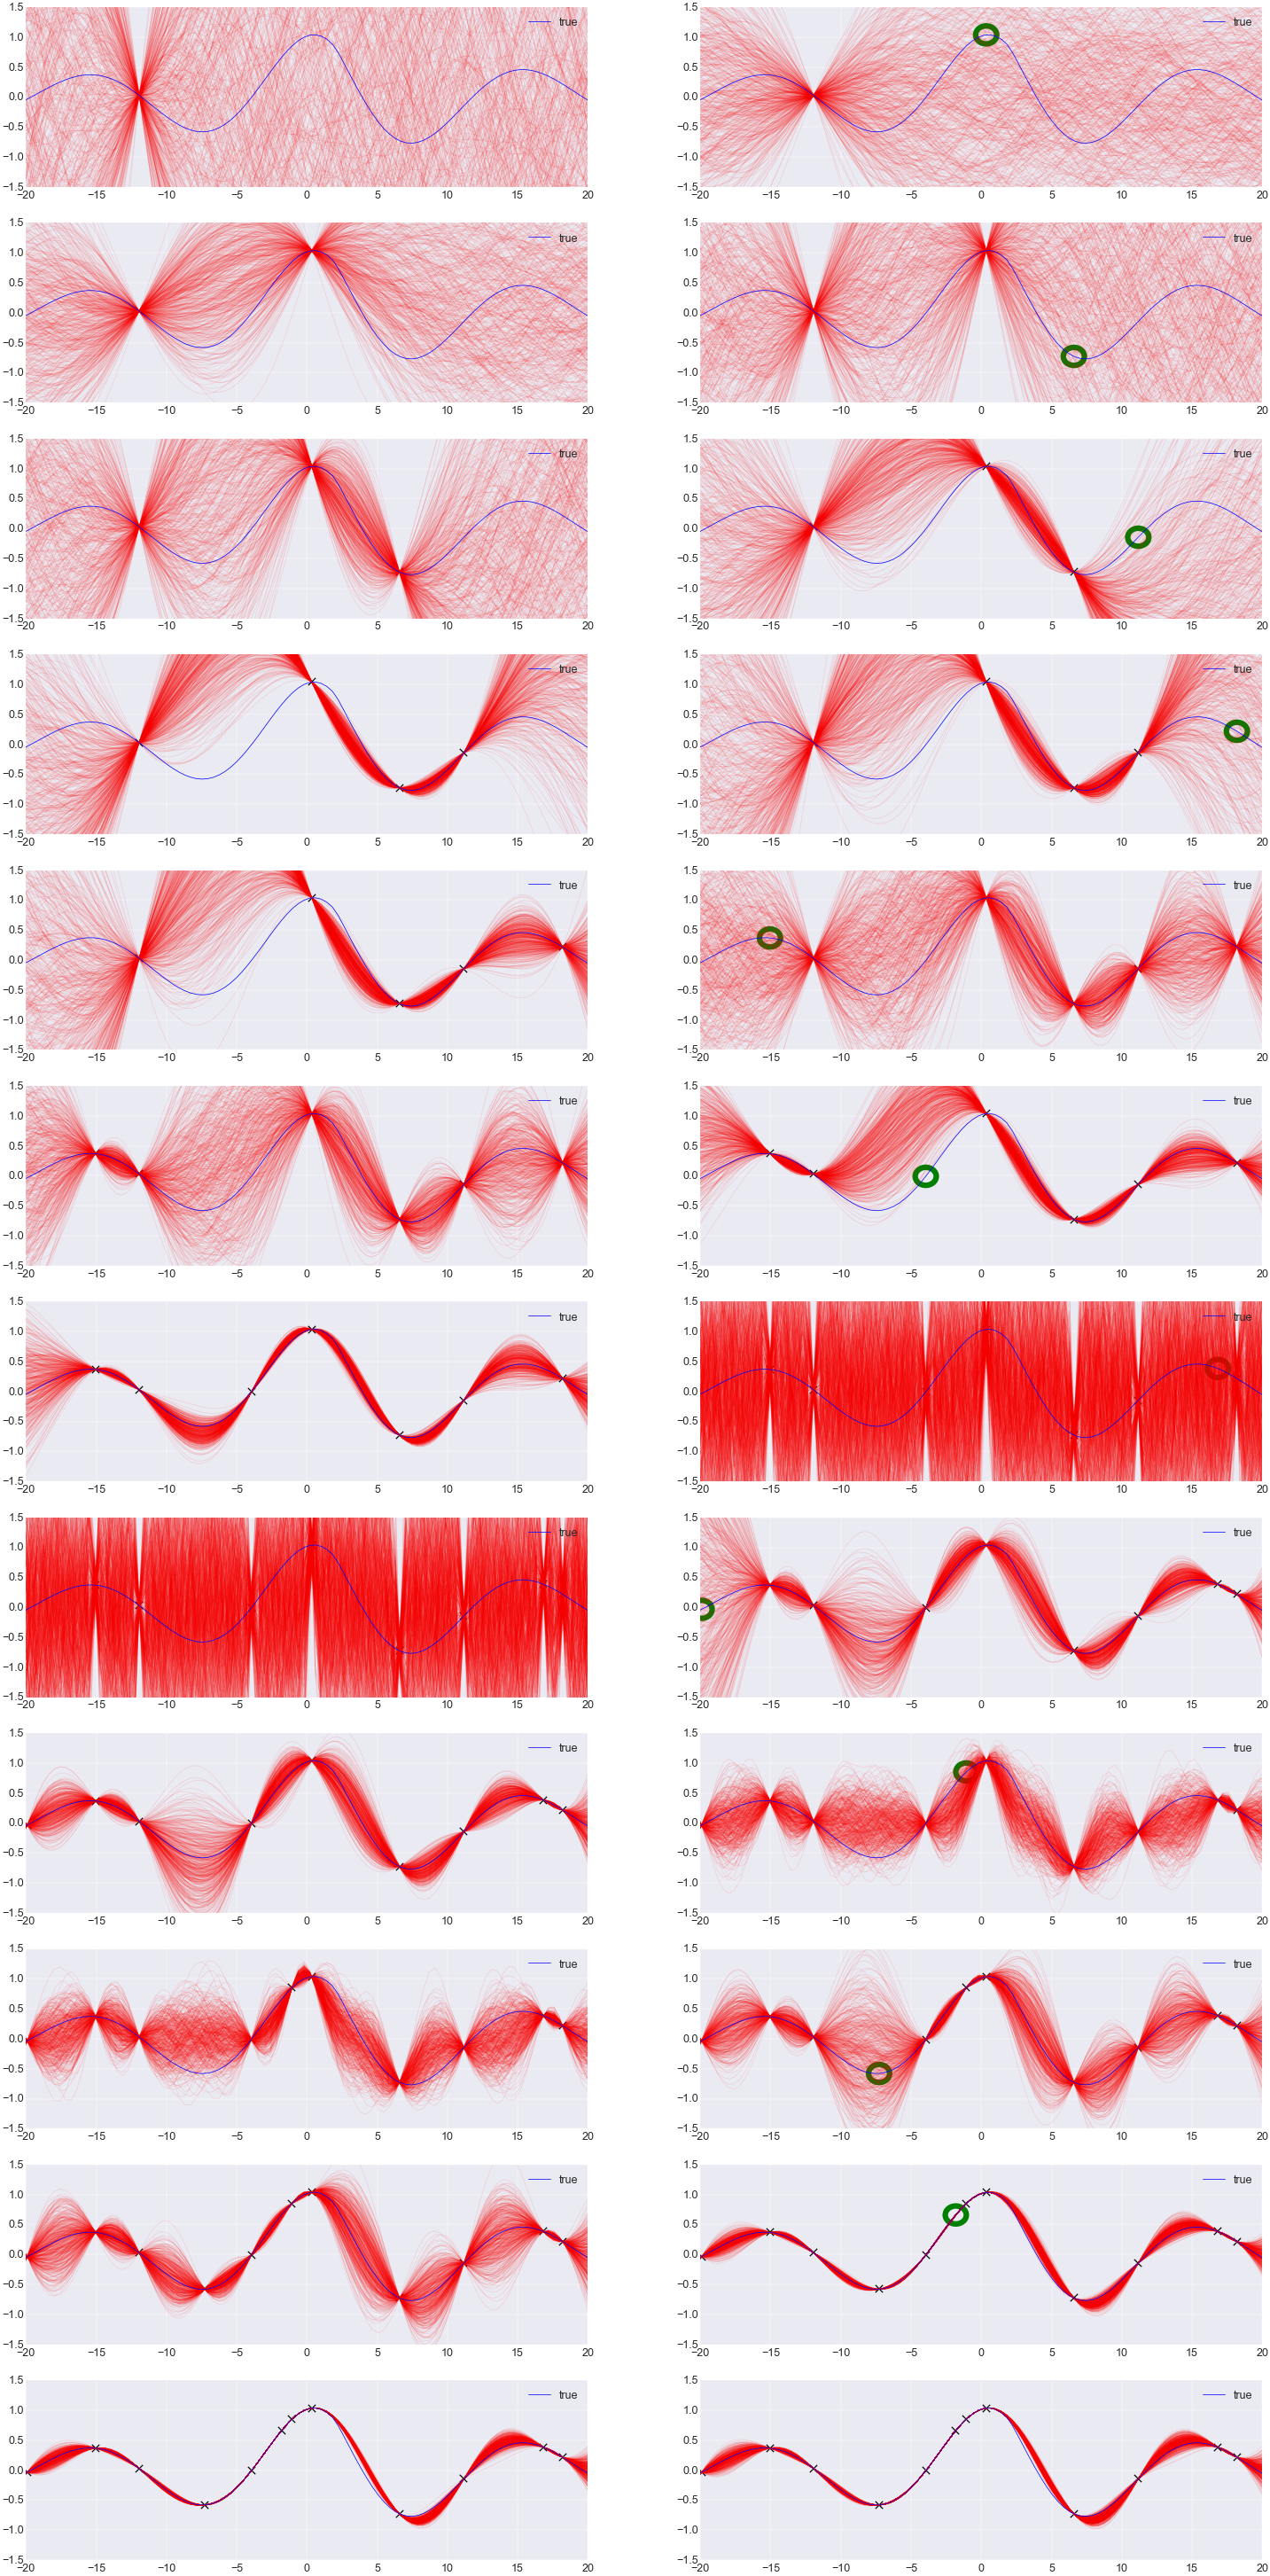
\includegraphics[height=0.8\textheight]{figs/BayesOpt_gpmem_sequence.png}
    \caption{
      Dynamics of Thompson sampling in Venture.
      The blue curve is the true function $V$, and the red region is a blending of 100 samples of the curve generated (jointly) by a GP-based emulator $V_\emu$.
      The left and right columns show the state of $V_\emu$ before and after hyperparameter inference is run on the new data, respectively.
      (We can see, for example, that after the seventh probe point, the Metropolis--Hastings sampler chose a ``crazy'' set of hyperparameters, which was corrected at the next inference step.)
      In the right column, the next chosen probe point is circled in green.
      Each successive probe point $a$ is the (stochastic) maximum of $V_\emu$, sampled pointwise and conditioned on the values of the previously probed points.
      Note that probes tend to happen at points either where the value of $V_\emu$ is high, or where $V_\emu$ has high uncertainty.
      }
    \label{fig:bayesopt-sequence}
\end{figure}
\end{comment}


%We consider a true and  unknown reward function $r(x)$ that we estimate with a GP prior $\mathcal{GP}(0,K(\mathbf{x},\mathbf{x}))$. We denote past observations with $\mathcal{D} = \{(x;

\FloatBarrier
\section{Conclusion}
We have shown Venture GPs. We have introduced novel stochastic processes for a probabilistic programming language. We showed how flexible non-parametric models can be treated in Venture in only a few lines of code. We evaluated our contribution on a range of hard problems for state-of-the-art Bayesian non-parametrics. Venture GPs showed competitive performance in all of them. 

\section*{Appendix}
\subsection*{A Covariance Functions}
SE and WN are defined in the text above, for completeness we will introduce the covariance:
\begin{equation}
k_{LIN}(x,x^\prime) = \theta (x x^\prime) 
\end{equation}
\begin{equation}
k_{PER}(x,x^\prime) = \theta \exp \bigg( \frac{2 \sin^2 ( \pi (x - x^\prime)/p}{\ell^2} \bigg) 
\end{equation}
\begin{equation}
k_{RQ}(x,x^\prime) =   \theta \bigg(1 + \frac{(x - x^\prime)^2}{2 \alpha \ell^2} \bigg)^{-\alpha}
\end{equation}

\subsection*{B Covariance Simplification}
\begin{minipage}{\linewidth}
\small
\belowcaptionskip=-10pt
\begin{lstlisting}[frame=single,mathescape,label=alg:simplify,basicstyle=\selectfont\ttfamily]

SE $\times$ SE                  $\rightarrow$ SE 
{SE,PER,C,WN} $\times$ WN       $\rightarrow$ WN
LIN $+$ LIN                $\rightarrow$ LIN
{SE,PER,C,WN,LIN} $\times$ C    $\rightarrow$  {SE,PER,C,WN,LIN} 
\end{lstlisting}
\end{minipage}
Rule 1 is derived as follows:
\begin{equation}
\begin{aligned}
\sigma_c^2 \exp(-\frac{(x-x^\prime)^2}{2\ell_c^2})  &=  \sigma_a^2 \exp(-\frac{(x-x^\prime)^2}{2\ell_a^2}) \times  \sigma_b^2 \exp(-\frac{(x-x^\prime)^2}{2\ell_b^2}) \\
&= \sigma_c^2 \exp(-\frac{(x-x^\prime)^2}{2\ell_a^2}) \times   \exp(-\frac{(x-x^\prime)^2}{2\ell_b^2}) \\
&= \sigma_c^2 \exp \bigg(-\frac{(x-x^\prime)^2}{2\ell_a^2} -\frac{(x-x^\prime)^2}{2\ell_b^2}\bigg) \\
&= \sigma_c^2 \exp \bigg(-\frac{(x-x^\prime)^2}{2\ell_c^2}\bigg) \\
\end{aligned}
\end{equation}
Rule 3 is derived as follows:
\begin{equation}
 \theta_c (x \times x^\prime) = \theta_a (x \times x^\prime) + \theta_b (x \times x^\prime) 
\end{equation}
For stationary kernels that only depend on the lag vector between $x$ and $x^\prime$ it holds that multiplying such a kernel with a WN kernel we get another WN kernel. Take for example the SE kernel:
\begin{equation}
 \sigma_a^2 \exp \bigg(-\frac{(x-x^\prime)^2}{2\ell_c^2}\bigg) \times  \sigma_b \delta_{x,x^\prime} =  \sigma_a \sigma_b \delta_{x,x^\prime}
\end{equation}
Multiplying any kernel with a constant obviously changes only the scale parameter of a kernel.
\newpage
\bibliography{May2015}
\bibliographystyle{apalike}
\end{document}
